\documentclass[master,english]{hgbthesis}
% Zulässige Class Options: 
%   Typ der Arbeit: diplom, master (default), bachelor, praktikum 
%   Hauptsprache: german (default), english
%%------------------------------------------------------------

% packages
\usepackage{pgfplots}
\usepackage{tikz}
\usepackage{color}
\usepackage{enumitem}
\usepackage{multicol}

% root folder of OMNeT++ installation
\newcommand{\omnetpproot}{/opt/omnetpp-4.6}

% hyphentation
\hyphenation{POWERLINK openPOWERLINK OMNeT cParsimSynchronizer cParsimProtocolBase cNullMessageProtocol cIdealSimulationProtocol cNoSynchronization cParsimCommunications parsim-communications-class}

% lstintputlistings style
\definecolor{xCodeComment}{RGB}{0,143,0}
\definecolor{xCodeWordStyle}{RGB}{216,33,174}
\definecolor{xCodeStringStyle}{RGB}{235,0,65}
\definecolor{xCodePreprocessor}{RGB}{130,71,33}
\definecolor{LightGray}{RGB}{240,240,240}

\lstset{language=C++,
    numbers=left,
    numberstyle=\tiny,
    basicstyle =\ttfamily\fontsize{8}{10}\selectfont,
    keywordstyle =\color{xCodeWordStyle},
    commentstyle = \color{xCodeComment},
    stringstyle = \color{xCodeStringStyle},
    showstringspaces = true,
    backgroundcolor=\color{white},
    framexrightmargin=2mm,
    breaklines=true,
    emph={\#endif},
    emphstyle={\color{xCodePreprocessor}},
    caption=\lstname,
    inputencoding={utf8},
    extendedchars=true,
    breaklines=true
}



\graphicspath{{images/}}    % name of directory containing the images
\logofile{FHOOeIntl2014}	% name of PDF, remove or use \logofile{} for no logo
\bibliography{literature}  	% name of the BibTeX (.bib) file

% disable colored borders for hyperlinks
%\hypersetup{
%    colorlinks=false,
%    pdfborder={0 0 0},
%}

%%%----------------------------------------------------------
\begin{document}
%%%----------------------------------------------------------

% Einträge für ALLE Arbeiten: --------------------------------
\title{Simulation and emulation of realtime communication networks}
\author{Franz Profelt}
\studiengang{Embedded Systems Design}
\studienort{Hagenberg}
\abgabedatum{2016}{05}{20}	% {YYYY}{MM}{DD}

%%% zusätzlich für eine Bachelorarbeit: ---------------------
\nummer{XXXXXXXXXX-A}   % XX...X = Stud-ID, z.B. 0310238045-A  
                        % (A = 1. Bachelorarbeit)
\semester{Sommersemester 2012} 
\gegenstand{Einführung in die Tiefere Problematik 1} 
\betreuer{Alois B.~Treuer, Päd.\ Phil.} % oder \betreuerin{..}

%%% zusätzlich für einen Praktikumsbericht: -----------------
\nummer{XXXXXXXXXX-B}   % XX...X = Stud-ID, z.B. 0310238045-B  
                        % (B = 2. Bachelorarbeit)
\betreuer{Mag.~Pjotr I.~Czar\\Creative Director}  % \betreuerin{..}
\firma{%
   Oligarchic Media International GmbH\\
   Online Division\\
   1020 Wien, Hubertusgasse 3a
}
\firmenTel{1-234-5678-100}
\firmenUrl{www.mogul.at}

%\strictlicense  % erzeugt restriktive Lizenzformel

%%%----------------------------------------------------------
\frontmatter
\maketitle
\tableofcontents
%%%----------------------------------------------------------

\chapter{Abstract}

\begin{english} %switch to English language rules
This should be a 1-page (maximum) summary of your work in English.
%und hier geht dann das Abstract weiter...
\end{english}

Im englischen Abstract sollte inhaltlich das Gleiche
stehen wie in der deutschen Kurzfassung. Versuchen Sie daher, die
Kurzfassung prä\-zise umzusetzen, ohne aber dabei Wort für Wort zu
übersetzen. Beachten Sie bei der Übersetzung, dass gewisse
Redewendungen aus dem Deutschen im Englischen kein Pendant haben
oder völlig anders formuliert werden müssen und dass die
Satzstellung im Englischen sich (bekanntlich) vom Deutschen stark
unterscheidet (mehr dazu in Abschn.\ \ref{sec:englisch}). Es
empfiehlt sich übrigens -- auch bei höchstem Vertrauen in die
persönlichen Englischkenntnisse -- eine kundige Person für das
"`proof reading"' zu engagieren.

Die richtige Übersetzung für "`Diplomarbeit"' ist übrigens
schlicht \emph{thesis}, allenfalls  "`diploma thesis"' oder "`Master's thesis"', 
auf keinen Fall aber "`diploma work"' oder gar "`dissertation"'. 
Für "`Bachelorarbeit"' ist wohl "`Bachelor thesis"' die passende Übersetzung. 

Übrigens sollte für diesen Abschnitt die \emph{Spracheinstellung} in \latex\ von Deutsch
auf Englisch umgeschaltet werden, um die richtige Form der
Silbentrennung zu erhalten, die richtigen Anführungszeichen muss
man allerdings selbst setzen %
(s.\ dazu die Abschnitte \ref{sec:sprachumschaltung} %
und \ref{sec:anfuehrungszeichen}).
			
% !TeX spellcheck = de_AT_frami

\chapter{Kurzfassung}
\begin{german}
Die Themengebiete der Simulation und Emulation gewinnen stetig an Bedeutung für die Entwicklung von eingebetteten Systemen. %TODO: find better phrase
Dies zeigt sich in der steigenden Nachfrage von umfangreichen Tests.
Eine Vielzahl von Anwendungsgebieten erfordern einen hohen Grad an Tests.

Dieser Trend führt zu einem steigendem Interesse an der Entwicklung einer Simulation oder Emulation für bestehende oder neu entwickelte Systeme.
Es existiert eine große Anzahl von verschiedenen Systemen zur Entwicklung von Simulationen die oftmals vielseitige Konfigurationsmöglich-keiten bieten.
Dieser Überfluss an verschiedenen Möglichkeiten eine Simulation zu entwickeln, kann Entwickler von der Entscheidung abhalten, eine Simulation für ihren Nutzen zu entwickeln.
OMNeT++ stellt ein sehr flexibles System zur Entwicklung von Simulationen für verschiedenste Anwendungen dar.

\begin{sloppypar}
Diese Arbeit analysiert den Aufbau und die Eigenschaften von OMNeT++ und zeigt die Möglichkeiten zur Konfiguration und Anpassung.
Es werden unterschiedliche Leistungsmessungen durchgeführt, die eine Testsimulation im Bezug auf Laufzeit, verarbeiteten Ereignissen und Echtzeiteigenschaften überprüft.
Es wurde ein optimierter Aufbau der Simulation gefunden, welcher zu einem verbesserten Ergebnis der Leistung führt.
Die vorhandenen Funktionen und die Möglichkeiten zur Entwicklung einer Echtzeitsimulation und Emulation stellt eine interessante Methode zum Testen und Entwickeln von eingebetteten Systemen dar. %TODO: find better phrase
Die Open Source Implementierung openPOWERLINK bietet die Möglichkeit, ein bestehendes Echtzeitkommunikationssystem zu analysieren und für eine Simulation anzupassen.
openPOWERLINK implementiert das weit verbreitete POWERLINK Protokoll, welches häufig im Bereich der Industrieautomation und Echtzeitkommunikation eingesetzt wird.
Bei der Entwicklung einer Simulation, die ein gegebenes System, wie die openPOWERLINK Implementierung, einbindet, werden Fragen bezüglich Mehrfachinstanzen aufgeworfen.
Es wurde eine Lösung für diese Problematik gefunden und anschließend eine Simulation entwickelt, die ein aus openPOWERLINK Knoten bestehendes POWERLINK Netzwerk nachstellt.
\end{sloppypar}
    
\end{german}
		

%%%----------------------------------------------------------
\mainmatter         % Hauptteil (ab hier arab. Seitenzahlen)
%%%----------------------------------------------------------

\chapter{Introduction}
\label{cha:introduction}
This thesis is intended to analyze the simulation framework \emph{OMNeT++} \cite{omnet_manual} and the possibilities for real-time simulation and emulation of a real time communication network.
A test simulation is analyzed for determining an optimized design regarding performance and real-time capabilities.
Furthermore a simulation of the real-time communication protocol POWERLINK and its open source implementation \mbox{openPOWERLINK} \cite{openpowerlink} is implemented. 
For developing this simulation the openPOWERLINK stack is analyzed and the platform dependencies are investigated.

\section{Motivation}
% needs and requirements for embedded systems
The fields of embedded systems and real-time communication entail critical requirements for timings and deterministic behavior.
The development of systems meeting those requirements can be very difficult due to the lack of possibilities for sufficient testing.
A variable testing environment is easing the development and verification of such systems.
The correct replication of complex scenarios and special operating conditions is not always possible.
Therefore the need for simulation is gaining importance with increasing complexity of embedded systems.

% real world simulation
Extended functionalities of simulation frameworks allows the usage as real-time simulation.
By simulating a system in real time, i.e. the simulated time passes according to the real (world) time, these simulations can be used in the fields of emulation and hardware in the loop (\emph{HiL}).
Which allow variable testing scenarios built with a simulated environment
These fields are necessary for testing embedded systems, due to the increased possibilities of testing scenarios and setups.

Because of the raising importance of simulation and emulation the analyze of simulation frameworks and the development of simulations for real-time communication systems represents an important field.

\section{Content}

% first chapters fundamentals and basics of OMNeT++, simulation, emulation, simulated designs, parallel simulation
The first chapters \ref{cha:omnet} to \ref{cha:parallel_sim} describe fundamentals regarding OMNeT++, general simulations, emulations and \emph{HiL}, simulation designs and parallel simulation.
These chapters should provide a extensive introduction and preparation for the further analyzes.

% development of a example network for design analyze and discussion of results
The following chapter \ref{cha:measurements} is analyzing two different fundamental designs and their impact on the achieved performance.
This performance is measured in multiple ways to analyze the simulation regarding runtime, processed events and real-time behavior.

% fundamentals of openPOWERLINK with focus on platform dependency and porting possibilities
Subsequently the Open Source stack openPOWERLINK is analyzed with special focus on the structure and the platform dependencies.
Shown in chapter \ref{cha:oplk}, these dependencies are used for the following development of an OMNeT++ simulation embedding the openPOWERLINK stack.
% approach to simulate openPOWERLINK in OMNeT++
This simulation and the implementation strategies are shown in chapter \ref{cha:porting}.

% resulting simulation and maybe performance
Simulating the openPOWERLINK stack obtains functional results, which are displayed in chapter \ref{cha:results}.

% conclusion
Finally the experiences and knowledge gained during this research are concluded and listed in chapter \ref{cha:conclusion}.

% appendix
The appendix contains three chapters and comprises code snippets form the OMNeT++ framework (\ref{app:omnetpp_code}), additional design measurements (\ref{app:measurements}) and some implementation samples of the openPOWERLINK simulation and the integration of the openPOWERLINK stack (\ref{app:simulation}).

\section{Purpose}
The purpose of this thesis is to analyze the OMNeT++ framework and its capabilities regarding real-time simulation.
Furthermore conducting an analyze of the openPOWERLINK stack focusing on the platform dependencies.
Which is leading to the development of a simulation embedding openPOWERLINK nodes within a simulation POWERLINK network.

This thesis shows the capabilities and strategies of developing a simulation for an embedded real-time communication network.
\chapter{OMNeT++}
\label{cha:omnet}

OMNeT++ represents an open source simulation framework written in C++.
It provides an object oriented modular discrete event network simulation framework.
The platform independent simulation library includes an integrated development environment (IDE), which is based on the Eclipse platform.
The commercial version OMNEST provides various licensing models, whereas OMNeT++ is only available for academic or non-profit use.
The intention of OMNeT++ is to provide infrastructure for writing simulations for various fields, especially those of network simulations.
For this thesis the latest version of OMNeT++ 4.6 was used and analyzed.

Simulations developed with OMNeT++ are based on different components, which provide functionality for communication and topologies.

\section{Components}
\label{sec:omnet_components}
Within an OMNeT++ simulation different components are used to represent the simulated system.
Each component is described by a \emph{network description} (NED) file and can be enhanced with C++ code.
The \emph{NED} file contains information about the component which is necessary for connecting and designing the simulated system, such as gates, submodules and parameters.

The different types of components and their usage are explained in the next sections.

\subsection{Network}
\label{sec:omnet_components_network}
The outermost component is a network which consists of other components like modules and channels.
The simulated topology and the connections between modules are defined within the network.
A network represents a closed system which can be simulated by itself, other components must be instantiated within a network to be simulated.
All instantiated modules, optional parameters and the connections between the modules are defined in the networks \emph{NED} file. \cite[section 3.2.1]{omnet_manual}

\subsection{Modules}
\label{sec:omnet_components_modules}
Modules represent functional groups of different complexities.
There are two types of modules available in OMNeT++.

A simple module is the smallest part within a simulated hierarchy and represents a functional unit.
For this functional unit the behavior for handling messages, the possible connections and additional parameters can be defined \cite[section 3.3]{omnet_manual}.
The possible connections of modules are represented by gates which can be connected to a channel or directly to other gates.

Multiple modules can be connected and combined to a compound module.
Such compound modules are used in the same way as simple modules, but represent bigger functional groups.
Compound modules are defined in the same way as networks, the instantiated submodules and the connections between them \cite[section 3.4]{omnet_manual}.
For OMNeT++ a network and a compound module is the same component which differentiate by the value for the built-in \emph{NED} property \emph{@isNetwork}.

An example network including simple modules connected to a compound module is shown in Figure \ref{fig:OMNeTComponents}.
Each module displayed in Figure \ref{fig:OMNeTComponents} defines two gates which is either an input, output or bidirectional gate.

\begin{figure}
    \centering
    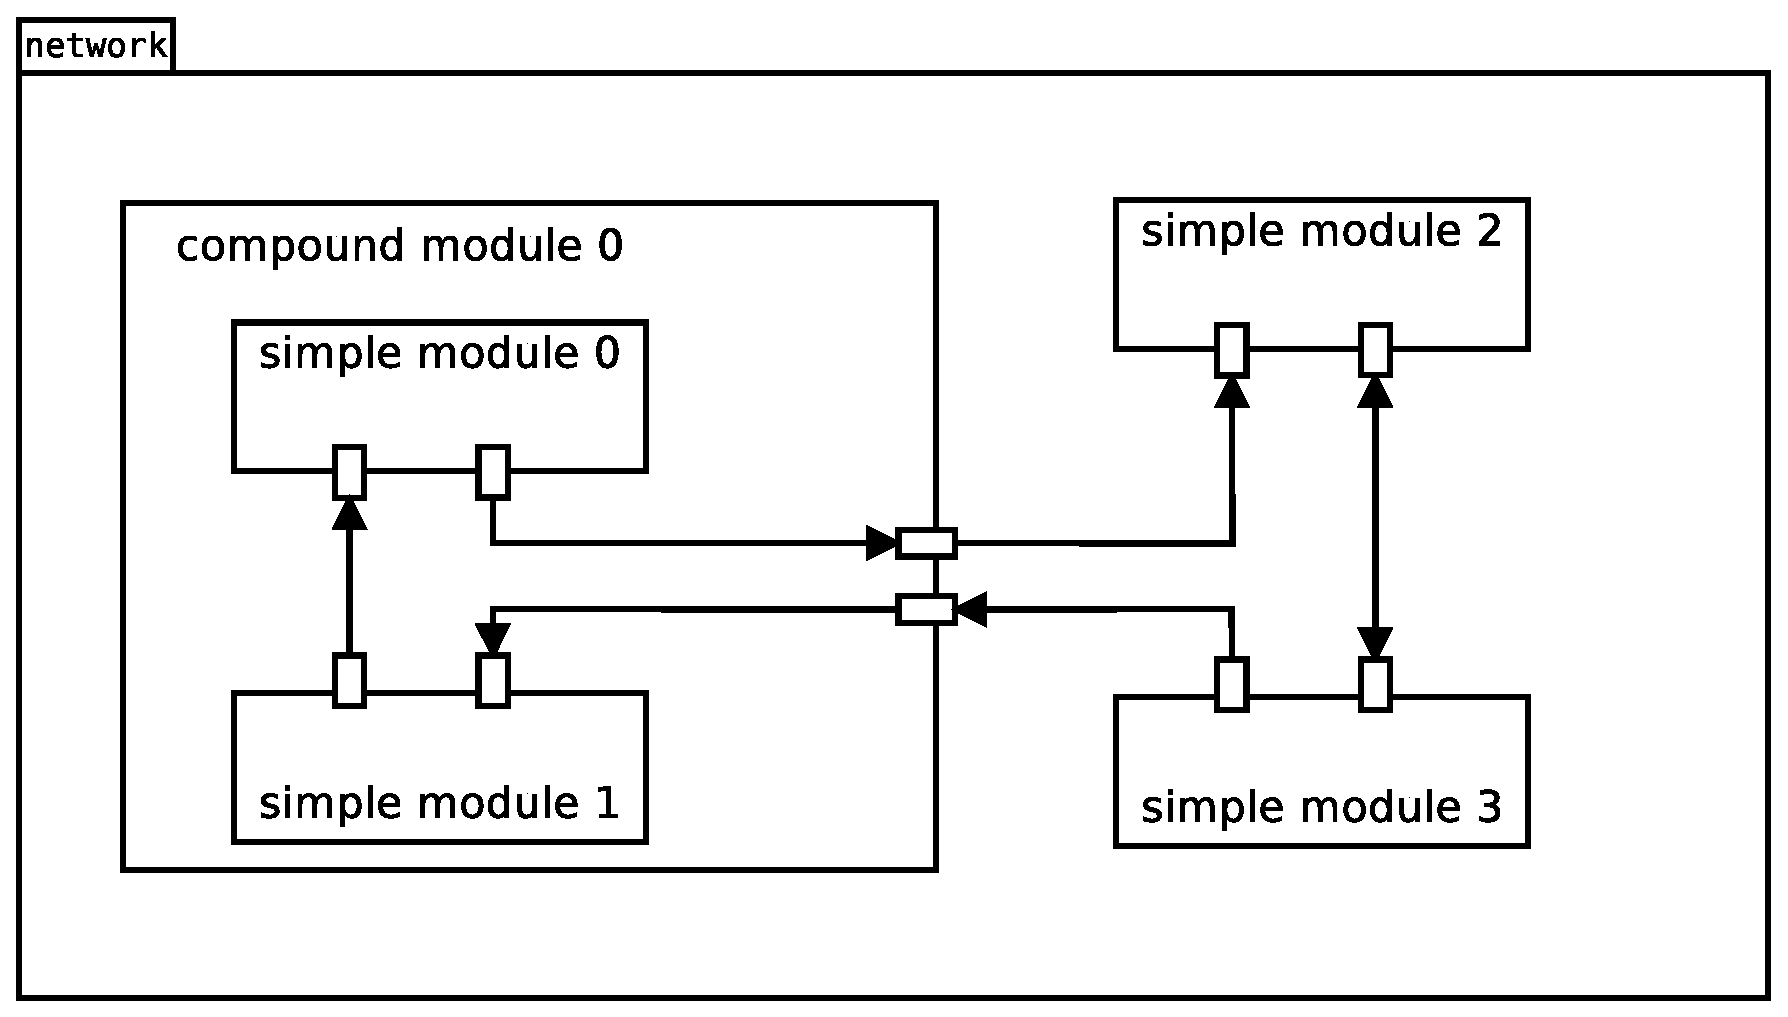
\includegraphics[width=0.9\columnwidth]{OMNeTComponents.eps}
    \caption{OMNeT++ components in an example network}
    \label{fig:OMNeTComponents}
\end{figure}

Specific functionality for custom components is implemented in the linked C++ code.
The assignment of \emph{NED} and C++ code is usually done with identical file names, but can also be done manually with the \emph{@class} \emph{NED} property.
The components can embed any functionality implemented in C/C++.
The usage of external libraries or language features is not limited, but must be used with care due to the effect on simulation performance.
For implementing the behavior of the modules and accessing the simulation environment, for example reading the value of a defined \emph{NED} parameter or sending a message via a gate, 
OMNeT++ provides different functionalities and strategies.

The functionality of a compound module is given by the submodules and their connections.
A simple module is implemented by overriding specific methods following one of the two strategies below:

\begin{itemize}
    \item Using the \emph{handleMessage} method, a module can react to incoming messages.
    Drawing on this strategy, the module is only active when a message is received.
    The methods \emph{send}, \emph{scheduleAt} and \emph{cancelEvent} can be used within \emph{handleMessage} for sending messages, scheduling self-messages and canceling of scheduled self-messages. \cite[section 4.4.1]{omnet_manual}
    
    \item The second strategy uses the method \emph{activity} and is also called \emph{process style} strategy.
    The method \emph{activity} is called by the simulation runtime as co-routine and can be implemented in the same way as a normal thread or process on an operating system.
    Returning from the \emph{activity} methods equals the finishing of the modules simulation.
    Beside the available methods of the first strategy, additional methods can be used within \emph{activity}.
    Using the method \emph{receive} the module waits until a message is received.
    Waiting for a specific amount of simulation time is achieved with the \emph{wait} method.
    A simple module using the \emph{activity} method is called as co-routine of the simulation core and is scheduled non-preemptively.
    I.e. the activity method is not interrupted by the simulation and has to suspend by itself.
    This is done by waiting for a received message or waiting for a specific amount of time. \cite[section 4.4.2]{omnet_manual}
\end{itemize}

\subsection{Channels}
\label{sec:omnet_components_channels}
The connections between modules can be realized in different ways.
A direct connection of two gates transports the transmitted messages immediately.
For applying transportation parameters (e.g. delay, latency, jitter) or implementing a custom behavior the connection can be established with a channel.
The OMNeT++ framework provides three built-in channels for direct usage or sub classing.

\begin{itemize}
    \item The \emph{IdealChannel} represents the same behavior as a direct connection between gates and transmits each message immediately.
    \item The \emph{DelayChannel} provides a \emph{delay} parameter for configuring a constant delay for each message.
    Additionally, there is the possibility to disable the channel and drop all containing messages.
    \item The \emph{DatarateChannel} provides the \emph{datarate} parameter for a variable rate of transmission including a configurable bit error rate (BER) and packet error rate (PER).
    These error rates can be used to mark a transmitted packet as erroneous.
\end{itemize}

These channels can be used directly or being subclassed for implementing custom functionality. \cite[section 3.5]{omnet_manual}

For implementing a custom channel, three methods must be implemented:

\begin{description}
    \item[isTransmissionChannel] returns true if the channel is a transmission channel, i.e. the transmission duration is calculated and set within the packet.
    This type of channel only affects messages of type \emph{cPacket} or derived types.
    \item[getTransmissionFinishTime] returns the finish time of the transmission for messages of type \emph{cPacket} or derived types.
    \item[processMessage] models the behavior of the channel and its functionality.
    In this method the results can be stored in a provided structure, which allows a dropping of the message and a change of the resulting transmission time.
    The transmitted message is passed to the \emph{processMessage} method, therefore various modifications can be made simulating the transmission through the channel. \cite[section 4.8]{omnet_manual}
\end{description}

\subsection{Parameters}
\label{sec:omnet_components_parameters}
Each component can define various parameters for configuration of their behavior.
The value of these parameters can be assigned in different ways.
The assignment from a \emph{NED} file can be done directly, via inheritance, or via a compound module or network which contains the component.
All parameters can also be set via a configuration file (e.g. omnetpp.ini) or interactively requested from the user.
In the case of none assignment a parameter can also define a default value.

These parameters can be used by the implemented behavior by using the \emph{par} method. \cite[section 3.6]{omnet_manual}

\subsection{Messages}
\label{sec:omnet_components_messages}
Transmitted data is encapsulated in another component called message.
Messages are a fundamental component of an OMNeT++ simulation as they do not only transport data but can also represent functional messages like jobs, events or tasks.
The meaning of a message depends on the written simulation and the simulated system. \cite[chapter 5]{omnet_manual}

These messages can also be customized for holding a specific set of data like a protocol header, checksum, or other specific data.
The existing message class \emph{cMessage} and its derived specialization \emph{cPacket} provide different members and methods which can be used for simulations.
These include control information, type information, time stamp, etc. and are included to ease the development of a simulation.
Adding a few simple data fields to a message can be either done by subclassing \emph{cMessage}, \emph{cPacket} or using the \emph{NED} language in special \emph{.msg} files.
By defining a custom message using \emph{NED} a customized subclass will be generated by the simulation and can be used as a normal message. \cite[chapter 6]{omnet_manual}

Any module can send a message via its gates by using the group of \emph{send} methods or send it to itself as \emph{self-message} with \emph{scheduleAt}.
The mechanism of messages is also used for implementing timeouts, timers, etc. by sending a specific message to the current module.
Therefore, the method \emph{scheduleAt} takes an absolute simulation time and a message as parameters and sends the given message at the given point of simulation time to the current module.
These \emph{self-messages} are handled by the same function as any other messages coming from other modules.
For the identification of \emph{self-messages}, the built-in method \emph{isSelfMessage} is available.
A scheduled \emph{self-message} can be canceled via the method \emph{cancelEvent} taking the scheduled message. \cite[section 4.7.1]{omnet_manual}

The \emph{send} method takes the message to send and the used gate as parameter.
For defining the gate, the defined name, the id or the object itself can be used \cite[section 4.7.2]{omnet_manual}.
When the transmission of the messages should occur at a later time, there is a built-in functionality given with the \mbox{\emph{sendDelayed}} method.
This method work in the same way as the default \emph{send} method but take an additional parameter which represents the delay. \cite[section 4.7.6]{omnet_manual}

Messages can also be sent directly to gates of defined modules without the need of a connection to the current module.
This is called \emph{direct sending} and can be useful when multiple sender modules send to a single input gate.
An example for this usage is shown in Figure \ref{fig:direct_sending}.

\begin{figure}
        \centering
        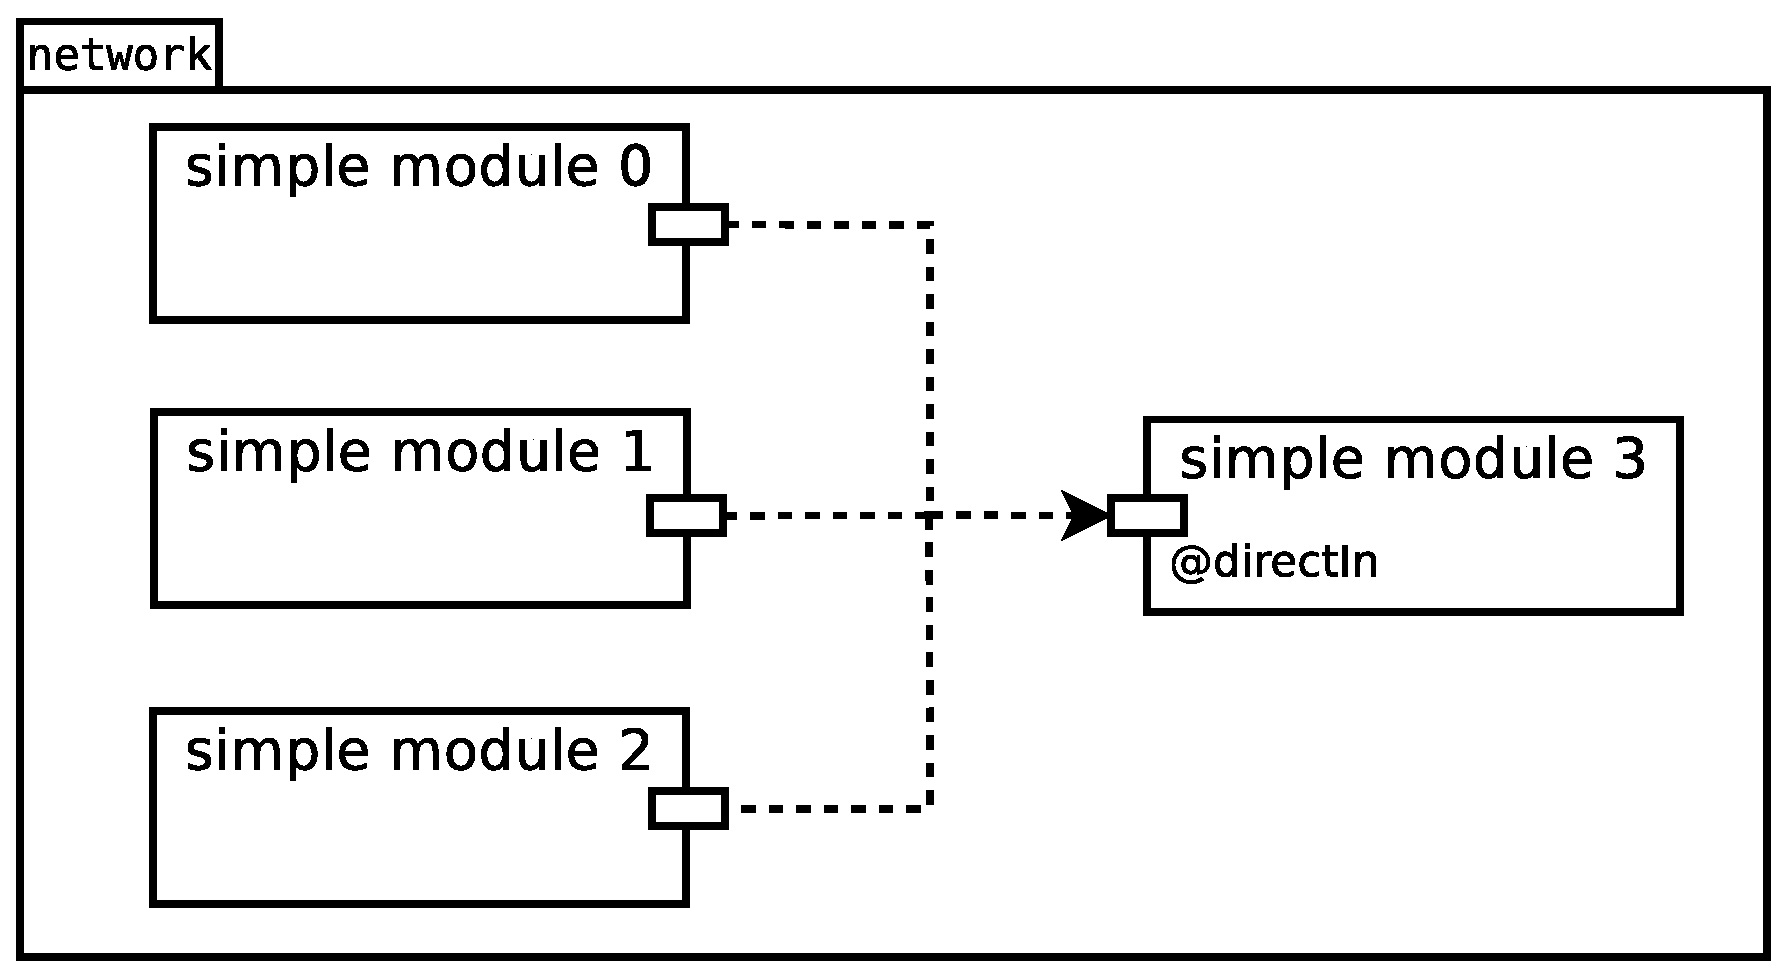
\includegraphics[width=0.9\columnwidth]{direct_message.eps}
        \caption{Multiple simple modules sending messages directly to simple module 3}
        \label{fig:direct_sending}
\end{figure}

Such a gate should be declared with the \emph{@directIn} \emph{NED} property to avoid notifications about a not connected gate. \cite[section 4.7.5]{omnet_manual}

Additional handling of messages as broadcasts and retransmission requires attention to the owner of messages.
By sending a message, its owner changes to both the simulation core and the receiver module.
Therefore, explicit copying of a message via \emph{dup} is necessary for sending a message to multiple modules or resending a message. \cite[section 4.7.3]{omnet_manual}

Each message sent either by another module or by the current module itself represents an event for the simulation with an according time, at which this event should happen, or the message should be delivered/received.
The execution and the handling of such events is done by the simulation core and defines the execution order and the performance of the simulation.
The different types of simulations and the simulation core of OMNeT++ are discussed in chapter \ref{cha:simulation}.


\section{Simulation results}
\label{sec:omnet_results}
The simulation of different systems results in different types of outcomes.
Therefore OMNeT++ provides multiple functionalities for recording and saving different results.


\subsection{Simulation library}
\label{sec:omnet_results_sim_lib}
The traditional way of recording simulation results is the use of the simulation library functions.

The built-in type \emph{cOutVector} provides the functionality used for recording a time series of data.
By holding an instance of \emph{cOutVector} a series of data can be recorded during simulation.
During initialization of the module the according name of the recorded time series should be set.
The recorded data of all \emph{cOutVector} instances is written at the end of the simulation to a single output vector file (\emph{.vec}). \cite[section 7.9.1]{omnet_manual}

Recording single values (scalars) is done, by using the \emph{recordScalar} method of a \emph{cModule}.
Usually this is called in the \emph{finish} method and may record a result of statistical analysis or even a whole statistic object.
All recorded scalars are written in a line based text file (\emph{.sca}). \cite[section 7.9.2]{omnet_manual}

The recording and the format of single vectors or single scalars can be defined in a configuration file as described in section \ref{sec:omnet_results_config}.

This method leads to an increased dependency of result recording and the simulated system due to the hard-coded implementation.
Since OMNeT++ 4.1 the newer strategies using \emph{signals} and \emph{statistics} are available and provide alternative methods for result recording.

\subsection{Signals and statistics}
\label{sec:omnet_results_signals}
The idea behind result recording using signals and statistics is the separation of data generation and recording.
The generated data is represented and distributed via signals.
The statistics access different signals for custom recording of required results. \cite[section 12.1.1]{omnet_manual}

Signals provide a functionality for a communication between modules which are not directly connected via their gates.
The usage of signals follows the \emph{publisher/subscriber} principle, i.e. modules can register callback objects to a specific signal.
If a new value for the signal is emitted, all registered callback objects are notified.

Signals are defined in the \emph{NED} file of the according module or channel and can be accessed by the defined name of the signal or the resolved signal id.
The name of a signal is defined globally, i.e. signals with identical names in different modules represent the same global signal.
A registered listener of such a global signal receives notification of all modules which emit a new value for their signal. \cite[section 4.14]{omnet_manual}

Using the \emph{@statistic} \emph{NED} property, the recording of data can be implemented using the built-in functionalities.
By defining a statistic property to a signal, a filewriter listener will be registered which records all notifications of this signal.
A statistic property provides multiple functionalities and options which can be defined in the \emph{NED} file.

Declaring a simple statistic property creates a signal with the according statistic name.
For separated configuration of signal and statistic, the \emph{source} option can be used to define a signal as the source of recorded data.
Built-in filters provide existing functionalities which can be directly embedded in the definition of the source signal.
For example, the \emph{count} filter can be used to count the notifications received on the defined signal.
Multiple filters can be chained for manipulating the receiving data.

The \emph{record} option defines what data shall be recorded by defining a recorder.
Recorders are the final elements of the recording chain, beginning at the source signal.
Between the source signal and the recorder, a variable number of filters can be set.
A single statistic can define multiple recorders resulting in multiple recorded data.
For distinguishing the importance of recorders, a question mark behind the recorder name can mark it as optional.
Optional recorders can be skipped by default, as described in section \ref{sec:omnet_results_config}.
The built-in recorders like \emph{last}, \emph{min}, \emph{max}, etc. result in an output scalar.
The recorder \emph{vector} results in an output vector.
This generated output container represent the same functionalities as the traditional recording methods described in section \ref{sec:omnet_results_sim_lib}.

There are various built-in filters and recorders available \cite[section 4.15.2]{omnet_manual} and there is also the possibility for writing and using custom filters and recorders. 
This can be achieved by subclassing \emph{cResultFilter} or \emph{cResultRecorder}. \cite[section 4.15.6]{omnet_manual}

The configuration of the resulting output (vector, scalar) is done independently of the used recording method.

\subsection{Configuration}
\label{sec:omnet_results_config}
The recorded results can be individually enabled and configured.
Therefore the configuration which data is recorded in which format is independent from the generated results and can be configured via a configuration file (\emph{.ini}).

The recording using signals and statistics provides more options and possibilities and therefore requires more different configuration methods.
Each statistic object can be configured individually using the \emph{result-recording-modes} for each statistic defined by its full path within the hierarchy.
This option defines the enabled recording modes (recorders described in section \ref{sec:omnet_results_signals}).
Additionally to the available recorders, the presets \emph{default} and \emph{all} are available.
The \emph{default} set contains all non-optional recorders, i.e. all recorders excluding recorders marked with a question mark.
The \emph{all} set contains all non-optional and optional recorders. \cite[section 12.2.1]{omnet_manual}

Statistics based recording consider a warm-up period which can be defined via \emph{warmup-period}.
Within this time beginning from the start of simulation no statistics will be recorded.
When using the simulation library to manually record results (cOutVector, recordScalar), the warm-up period must be considered manually. \cite[section 12.2.2]{omnet_manual}

The resulting output files can be defined independently from the used recording method via the options \emph{output-vector-file} and \emph{output-scalar-file}. \cite[section 12.2.3]{omnet_manual}

The configuration of the recording via the simulation library (section \ref{sec:omnet_results_sim_lib}) is done by \emph{scalar-recording}, \emph{vector-recording}, \emph{vector-recording-interval} and \emph{vector-record-eventnumbers}.
These options allow the dis- or enabling of specific output vectors and scalars given by their full path within the hierarchy.
For vector recording the definition of specific recording intervals is possible to record only interesting intervals.
Also the addition of the event number to the output file can be dis- or enabled.
These options also affect the recording via signals and statistics because the statistic property generates output vectors and scalars. \cite[section 12.2.4, section 12.2.5]{omnet_manual}

\section{Running an OMNeT++ simulation}
\label{sec:omnet_running}
The output of the OMNeT++ build process is by default an executable for starting the simulation.
All generated simulation executables provide command line parameters for the configuration of specific simulation runs.
The most important parameter can be passed directly or via the \emph{-f} command and defines the used configuration files for the simulation run.
The configuration files and some key options for running a simulation are described in section \ref{sec:omnet_running_config}.

Within a configuration file multiple configurations can be defined and the configuration which should be used for simulation can be defined via the \emph{-c} command line option.
If no configuration to load is specified but multiple configurations are defined within the configuration file, the behavior depends on the started user interface.
Starting the graphical user interface will prompt the user to choose a configuration.
The command line user interface will execute the general configuration.

The configuration of the path to load the \emph{NED} files can be defined within a configuration file as well as by a command line option (\emph{-n}).
With multiple configurations, the values are merged into a combined load path.

The selection of the user interface can be defined via the command line option \emph{-u}.
This definition overrules a configured default user interface of a configuration file.
The different user interfaces and their functionalities are shown in sections \ref{sec:omnet_running_tkenv} and \ref{sec:omnet_running_cmdenv}.

OMNeT++ also provides the \emph{opp\_run} tool, which is basically an empty simulation.
With this tool, a simulation model which is built as shared library can be started.
With \emph{opp\_run} or any other simulation executable all available command line options and their description are acessable via \emph{-h}.

Further configuration options of the configuration file can also be set via the command line interface by preceding the option with \emph{-{}-}.
If a double configuration occurs, the via command line parameter passed value will be preferred. \cite[section 10.1.1, section 10.1.2]{omnet_manual}

\subsection{Configuration}
\label{sec:omnet_running_config}
The configuration file can be given by a command line parameter, usually the file \emph{omnetpp.ini} is used.

Within a configuration file, multiple configurations or sections can be defined.
When starting a simulation, the loaded configuration can be set, therefore multiple different simulation runs with different configurations can be defined within a single configuration file. \cite[section 9.2]{omnet_manual}

The most essential configuration is the simulated network which is defined by the name of the according \emph{NED} network.

The duration of the simulation can be defined via an ending simulated system, i.e. modules which automatically finish their execution, or a time limit is defined.
A time limit can either be defined for the simulation time (\emph{sim-time-limit}) or the cpu time (\emph{cpu-time-limit}).

The behavior of the simulation in case of errors and the connection behavior of debuggers can be defined via various options as \emph{debug-on-errors}, \emph{debug-attach-on-error}, etc.. \cite[section 10.1.3]{omnet_manual}

Specific configuration for the command line user interface are available for controlling the output of a running simulation (\emph{cmdenv-express-mode}, \emph{cmdenv-status-frequency}, \emph{cmdenv-perormance-display}) and the possibility of user interaction (\emph{cmdenv-interactive}).
The effects of these options are shown in section \ref{sec:omnet_running_cmdenv}.

Parameters of loaded components can be set individually, commonly set via wildcards, or requested from the user.
Values which are directly set within the \emph{NED} files can not be overwritten by a configuration file.
Therefore a more flexible simulation model provides the majority of parameters via configurations.
Parameters of modules can either be set individually by the full path within the simulated hierarchy or commonly set via wildcards. \cite[section 9.3]{omnet_manual}

\begin{sloppypar}
The configuration of module parameters also allow the definition of value ranges for so-called \emph{parameter studies}.
These \emph{parameter studies} result in multiple simulation runs iterating over all specified parameters.
Simulating a specific iteration, can be achieved via setting the run number passed by command line interface (\emph{-r}) or defined in the configuration (\mbox{\emph{cmdenv-runs-to-execute}}). \cite[section 9.4]{omnet_manual}
\end{sloppypar}

Defined via the command line parameter or via the \emph{user-interface} option, different user interfaces can be used to start and visualize the simulation.

\subsection{Graphical user interface \emph{Tkenv}}
\label{sec:omnet_running_tkenv}
OMNeT++ provides the graphical environment \emph{Tkenv} for running and visualizing simulations.
\emph{Tkenv} provides various different possibilities for a graphical presentation of the simulated network, processed events and simulation results.

This user interface is useful for developing and debugging a simulation during the development.
The possibilities to inspect each component within the simulated system provide deep insight to the simulated system.

Different possibilities for graphical representation of the system and animation of progress/results allow a convenient presentation of a simulated system.
This presentation allows for educational and presentational purposes of the simulation. \cite[section 7.1]{omnet_user_guide}

Running complex simulations with multiple parameter studies is not recommended within Tkenv due to the increased overhead for refreshing the representation.
Different run modes (\emph{normal run}, \emph{fast run}, \emph{express run}) allow skipping of user interface updates. \cite[section 7.3.2]{omnet_user_guide}

For simulations with increased complexity and longer simulation durations the command line user interface \emph{Cmdenv} should be preferred.

\subsection{Command line user interface \emph{Cmdenv}}
\label{sec:omnet_running_cmdenv}
The \emph{Cmdenv} environment represents a command line user interface.
Using this environment, no graphical user interface is shown, or will be updated.
This simulation method is recommended for batch simulations or running simulations with increased complexity and no need for graphical representation due to the improved performance.

\begin{sloppypar}
During a running simulation within \emph{Cmdenv} the output printed to the command line depends on the configuration.
For debugging purposes, the \emph{normal mode} can be used and detailed event information will be printed to the command line.
When running simulations over a longer period of time, the \emph{express mode} is recommended and only periodically status updates will be printed.
The frequency of the updates and the printed details can be configured via the \emph{cmdenv-status-frequency} and the \mbox{\emph{cmdenv-performance-display}} options. \cite[section 10.2.3]{omnet_manual}
\end{sloppypar}

Simulations defining one or more parameter studies result in multiple runs which can be defined via a command line parameter or in the configuration.
For executing multiple runs, OMNeT++ provides the \emph{opp\_runall} tool which starts each run in a separate operating system process.
Using multicore/multiprocessor systems \emph{opp\_runall} can execute different simulation runs on different cores/processors. \cite[section 10.4.3]{omnet_manual}
\\

Running the simulation within \emph{Tkenv} or \emph{Cmdenv} executes it by default sequentially.
Parallel simulation imposes different requirements on the simulated systems and its design.
These requirements and the functionality of parallel simulation is analyzed in chapter \ref{cha:parallel_sim}.

\section{Simulation Core}
Simulations based on OMNeT++ are designed and simulated as discrete event simulations (\emph{DES}).
The characteristics of the \emph{DES} and the comparison to other types of simulation are discussed in the chapter \ref{cha:simulation}.

Details about the different simulation properties and functionalities are outlined in section \ref{sec:simulation_omnet}.
\chapter{Simulation}
\label{cha:simulation}

A Simulation attempts to replicate and forecast the behavior of real world systems.
Such a replication is used in various fields for testing and verifying theories and systems.
The field of simulation steadily gains importance, due to the increasing complexity of systems; e.g. embedded systems and real-time systems.
Especially the development and testing of real-time communication systems can essentially be improved by using simulation and emulation techniques.

Different types of simulation are applicable for different types of simulated systems and aimed results.
Differences are shown in the processing of the simulated systems and in the handling of simulation time.
\cite[section 1.2]{mchaney2009understanding}

\section{Continuous simulation}
\label{sec:simulation_cont}
Continuous simulations handle uninterrupted values over a simulated time range.
This behavior may be determined by equations describing the system.
For correct simulation of a continuous system the model must be executed for the whole simulated time range.
These simulations are usable for scenarios when the temporal behavior of the simulated models is of interest. \cite[section 1.2.1]{mchaney2009understanding}

Simulations and testing scenarios in the field of real-time communication are based on discrete events at specific points in time, e.g. the reception of data.
The continuous processing of occasions between events is often not necessary, therefore a discrete event simulation (\emph{DES}) is more applicable.

\section{Discrete event simulation}
\label{sec:simulation_event}
This type of simulation is based on processing discrete events.
During the processing of events the simulation time does not advance and the required processing time is not considered in simulation time.
The simulation time is advancing with multiple processed events and their defined point in simulation time.
Between two consecutive events neither any processing is done nor changes of the system state are occurring. \cite[chapter 1]{matloff_introduction_2008}

The assumption is that none, for the simulation relevant, events are happening between two consecutive events.
This exclusion is done by the implementation of the simulated model and must be concluded with care to the intention of simulation.
Simulating a real world system therefore requires the filtering of occasions for focusing on the simulation goal. \cite[section 4.1.1]{omnet_manual}

The implementation of a \emph{DES} can be done in various ways using different strategies or paradigms.
In \cite[chapter 2]{matloff_introduction_2008} Matloff introduced different paradigms to realize a \emph{DES}.
Using OMNeT++ the \emph{Event-Oriented Paradigm} and the \emph{Process-Oriented Paradigm} are applicable and can be achieved as following:

\begin{itemize}
    \item The usage of the \emph{handleMessage} method matches the \emph{Event-Oriented Paradigm} and allows event based development.
    \item The \emph{Process-Oriented Paradigm} can be realized by using the \emph{activity} method and represents the \emph{process style} strategy.
\end{itemize}

\begin{sloppypar}
The \emph{Activity-Oriented Paradigm} could also be implemented within OMNeT++ by using either the \emph{activity} or the \emph{handleMessage} method.
This paradigm would require the implementation of a custom polling module which checks regularly for new events or monitors the activity of other modules.
This implementation would replace and bypass the handling and scheduling of messages in OMNeT++ and is not recommended. \cite[chapter 2.1]{matloff_introduction_2008}
\\
\end{sloppypar}

The above discussed types of simulations belong to the group of \emph{offline simulations} i.e. the simulation time is not connected to the processing time.
Approaching the fields of emulation and \emph{HiL} such a connection is necessary and the behavior of \emph{offline simulations} is unusable.
These fields demand the type of real-time simulation.  \cite[section III.B]{belanger_what_2010}

\section{Real-time simulation}
\label{sec:simulation_real_time}
Real-time simulations change the meaning of simulation time and add a connection to the real-time.
The simulated events should be executed at the correct time to match the real-time.
In this context the real-time represents the real world time, cpu time, or wall time, i.e. the time which passes for the real world during the execution of the simulation.
Running a real-time simulation results in processing a simulated second within an elapsed real world second.
This type of simulation is not possible for every simulated system as the limits are defined by the time required to execute the operations specified by the model.

The achieved execution speeds are strongly depending on the following factors:
\begin{description}
    \item[Model] The complexity of the simulated model, i.e. the functionality to process events affects the achievable execution speed.
                 Simple functionalities can be executed faster than complex library calls or nested functions.
    \item[Host system] The properties of the host system used for running the simulation define the possible execution capabilities and therefore the performance of the executed simulations.
                       This dependency is described in section \ref{sec:simulation_requirements}.
\end{description}

If the execution of the model behavior for reacting to an event takes more processing time than the simulated duration (timespan to next event), the simulation lags behind the real world behavior.
Such an erroneous behavior must be corrected by the simulation core by speeding up the simulation, for example by decreasing idle times between events.
The correction of such behavior results in an increased jitter (variance of event execution time).
\cite[section III.B]{belanger_what_2010}

The quality of the real-time simulation is strongly depending on the simulated system and its composition.
Therefore the ideal results can be achieved by analyzing the simulated system regarding the real-time requirements and processed events.
An example of such an analysis and the modifications of an OMNeT++ simulation for timing improvements are shown in \cite{scussel_improvements_2015}.

The existing functionalities and properties of a simulation using the OMNeT++ framework is shown in the next section.

\section{Simulation with OMNeT++}
\label{sec:simulation_omnet}
By default simulations developed with OMNeT++ are discrete event based simulations.
This behavior is defined by the scheduler and the simulation core, which can be tailored by using custom components. \cite[section 4.1]{omnet_manual}

Within OMNeT++ each event is represented by a message with a defined \emph{arrival time}.
Events are created by modules and then inserted in the so called future event structure (\emph{FES}).
The simulation core executes all events within the \emph{FES} at the according simulation time.

The scheduler is the main part of the simulation core for controlling the event handling the execution order.
The scheduler accesses the \emph{FES} and chooses the next event to be handled by the simulation.
The class \emph{cScheduler} represents the interface which is required for an event scheduler usable in OMNeT++.
By default the derived class \emph{cSequentialScheduler} is used.
This scheduler implements the default discrete event based simulation and handles the events according to their execution time, scheduling priority and scheduled time.
The scheduling priority provides a mechanism for controlling the execution order of multiple events at the same time. \cite[section 4.1]{omnet_manual}.

An exemplary approach to realize the type of real-time simulation is implemented in the \emph{cRealTimeScheduler}.
This scheduler executes the events according to their planned arrival time.
The arrival time of the next event is compared with the current real time.
When the simulation is ahead of the real time, the simulation is paused for the remaining time.
The \emph{cRealTimeScheduler} waits in hard-coded 100 ms chunks for allowing a responsive simulation including graphical updates.
This provided scheduler does not handle a lagging simulation in a special way and simply skips the waiting times within the method \emph{getNextEvent}. 
The definition and implementation of the \emph{cRealTimeScheduler} are shown in the appendix section \ref{app:omnetpp_code_real_time_scheduler} or in the OMNeT++ API \cite[cRealTimeScheduler]{omnet_api}.

For emulations and \emph{HiL} this concept is not applicable, because the communication with real components does rarely contain static sleep times.
The OMNeT++ sample \emph{sockets} demonstrates this problem and a possible solution with a custom scheduler implementing the \emph{cScheduler} class.
The custom scheduler \emph{SocketRTScheduler} and its functionality is further analyzed in section \ref{sec:emulation_omnet_existing}.

% omnet++ real time handling/correction
Handling a simulation which is faster than the real world system can be done in various ways as demonstrated by \emph{cRealTimeScheduler} or the \emph{SocketRTScheduler}.
If the simulation is lagging behind the real-time, the scheduler must try to speed up the simulation and catch up to the real time.
The task of catching up to the real-time is very difficult for complex simulations with tight timings.
If the simulation lags constantly behind the real world using the \emph{cRealTimeScheduler} it becomes a discrete event based simulation and no real-time simulation is possible.

The sample scheduler provided by \emph{cRealTimeScheduler} and \emph{SocketRTScheduler} can lead to the correct strategy of implementing an optimized scheduler.

To validate a real-time simulation regarding timing quality the performance ration can be used.
This ratio represents the simulated seconds per real time seconds.
A lagging simulation is defined by a performance ratio of less than one and simulation which simulates faster as the real time shows a ratio greater one.
The goal of a real time simulation is a constant ratio of one.
The process of catching up of a lagging simulation to achieve a performance ratio of one can also influence the general timing behavior.
Therefore the variation of delays (jitter) increases when the simulation lags temporarily.
For emulations or the fields of \emph{HiL} an increased jitter for a signal can be very critical and must be analyzed carefully.

The host machine for the simulation and its components affect the achieved simulation times.
The dependencies of the host system and the results of existing researches is shown in section \ref{sec:simulation_requirements}.

Developing the simulation of a given system results in the situation of existing code.
This code must be encapsulated in different modules and be executed depending for incoming messages and thereby creating new message for sending.
Given systems can be designed in various hierarchies in sight of number of modules and complexity of simple modules.
The different designs and their effects on real time simulation is shown in the chapter \ref{cha:design}.

\section{System requirements}
\label{sec:simulation_requirements}
The host system for the simulation is very important regarding speed and performance of a simulation and therefore the achievable timings of a real-time simulation.
The limitations of achievable timings of a real-time simulations are defined by the execution speed of the simulated model plus the time for executing the simulation functionality around it.
Assuming the \emph{RAM} (random access memory) of the host systems is large enough to hold the complete simulation code and data, the limit is defined by the execution speed of the code.
Which is affected by the \emph{CPU} (central processing unit) capabilities and the speed of connected memories.
These memories include the \emph{RAM}, every cache and register which is used for holding simulation code and data.
The evolution of simulations and real-time simulations arises from analog simulations, to digital simulations running on supercomputers and currently common simulations running on commercial of the shelf (\emph{CTOS}) systems and field programmable gate arrays (\emph{FPGA}).
This evolution provides more computing capabilities for lower costs. \cite[section IV]{belanger_what_2010}
\chapter{Emulation and Hardware in the loop}
\label{cha:emulation}

The field of emulation is strongly related to the field of simulation and targets the imitation of real world systems.
In contrast to a simulation the purpose of an emulation is to replicate a real world system and providing the possibility to interact with other components in the same way as the emulated system ought to.
Emulation is used in various fields reaching from the replication of outdated computer systems for executing old applications, to the field of \emph{HiL} (hardware in the loop) and the usage for verification and testing of embedded systems. \cite{emulation_koninklijke}

The fields of emulation and \emph{HiL} are based on real-time simulations combined with a connection to the real world.
The replication of a given environment allows to enclose a specific component and then execute specific scenarios.
Such a component can either be a software application (\emph{SiL} - software in the loop) or hardware component (\emph{HiL}).
This connection of simulated systems with real systems can be used for testing and verification of systems under development.
An emulation system running on a host system and an enclosed system under test is shown in figure \ref{fig:emulation_overview}.
The shown structure is typical for various types of emulations with different enclosed systems.

%TODO: check figure
\begin{figure}
\centering
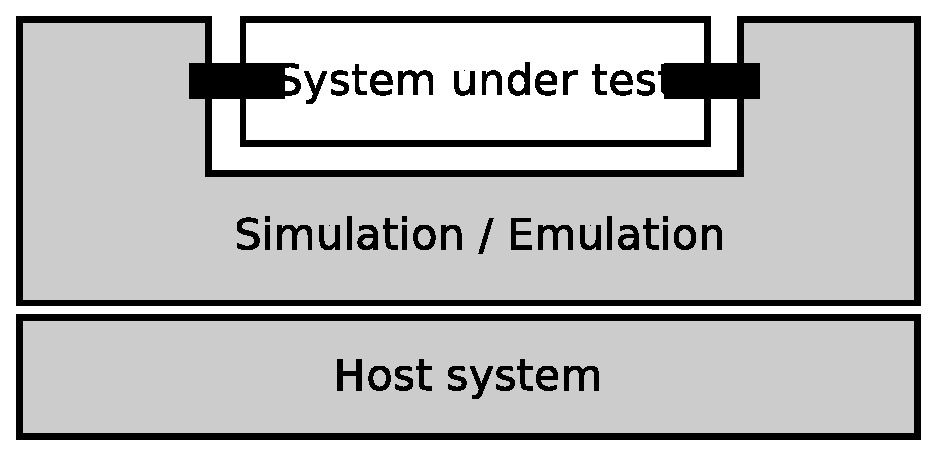
\includegraphics[width=0.7\linewidth]{images/emulation_overview}
\caption{Overview of an emulation environment running on a Host system (gray) with an enclosed system under test (white) and the connections between those systems (black).}
\label{fig:emulation_overview}
\end{figure}



Such a test method can test various different scenarios due to the flexibility of the simulated system.
\cite[section I]{lu_low-cost_2007}

The used simulation can be realized with any simulation technology and existing simulation frameworks, as long as the execution as real-time simulation (described in section \ref{sec:simulation_real_time}) is possible.
The requirement of real-time simulation must be met for specific given response times to allow the valid interaction with external components.
In the following section the capabilities regarding emulation and \emph{HiL} provided by the OMNeT++ framework are discussed and analyzed.

\section{Emulation and \emph{HiL} using OMNeT++}
\label{sec:emulation_omnet}
For the fields of emulation and \emph{HiL} OMNeT++ provides customizable components within the simulation core and thereby allows different strategies for implementing the required behavior.
The built in functionalities and their usage shown in given examples are explained in the following section.

\subsection{Existing functionality}
\label{sec:emulation_omnet_existing}

The sample simulation \emph{sockets} shows the possibilities and methods for developing an emulation.
This example simulates a web server with a dynamic number of clients.
For exemplary usage as emulation an external client can also be used, which represents the connection to the real world and communicates with real requests by the user.
These interaction is established via the connection to a local address and the hyper text transfer protocol (\emph{HTTP}) GET request by a web browser.
This emulation uses the custom scheduler \emph{SocketRTScheduler}, which is implemented similar to \emph{cRealTimeScheduler} and derived from \emph{cScheduler}. \cite{omnet_api}
The custom scheduler holds a TCP socket for communication with the real world.
During wait times the schedule listens to the network interface and converts receiving data to simulation events.
These generated events are distributed by the \emph{ExtHttpClient} or \emph{ExtTelnetClient}.
These simple modules represent the external real world components within the simulated network.
The implementation can be found within the \emph{sockets} sample included in the OMNeT++ framework or in the appendix section \ref{app:omnetpp_code_socket}.
This behavior is feasible for this exemplary usage, but if the timings of the simulated systems sharpen this scheduler would not allow sufficient communication.
Analyzing the implementation and the achievable timings lead to different possibilities for optimizations as described in \cite{scussel_improvements_2015}.

The combination of a real-time simulation and a real world system requires a connection between them.
Such a connection can be established using various functionalities, but must always fulfill the functionality of converting occasions form the real world to simulation events and vice versa.
This connection affects the achievable performance and the temporal behavior of the simulated components respectively to the real world component.
In the \emph{sockets} example the built in functionalities for sending and receiving data via sockets are used.
These built in functionalities are implemented depending on the host platform OMNeT++ was built and are therefore using either the \emph{WinSock2} library on Windows operating systems or otherwise the Unix socket implementation.
These built in functionalities for socket communication are located in the \emph{include/platdep} folder within the OMNeT++ installation.
In section \ref{sec:emulation_communication} different strategies and recommendations regarding the communication implementations are discussed.

\section{Communication with the real world}
\label{sec:emulation_communication}
For the fields of emulation and \emph{HiL} the communication with the real world is very important and affects the achievable performance.
By encapsulating all used communication functionalities in specific modules the simulated model can be clearly separated.
Using OMNeT++ the separated communication components can be realized with modules implementing the connection functionalities or customizing simulation components such as a custom scheduler.
Recommended implementation strategies for each communication functionality and their properties are discussed in the following sections.

\subsection{Receiving}
\label{sec:emulation_communication_receiving}

The receiving component can be implemented as a simple module using the \emph{process style} strategy.
This strategy allows an intuitive implementation observing the interface, then creating messages with the received data and sending them to the simulated system.
Executing the simulation sequentially does not allow constant listening by such a receiver module, therefore this must be interrupted to allow the execution of the remaining simulation.
Using parallel simulation described in chapter \ref{cha:parallel_sim} the receiving module can be implemented blocking.
Assigning the receiving module to a single processor allows a constant listening to the communication interface.
This represents an improved behavior and extended possibility for handling real time occasions and provides a potential lowered delay for the event conversion.

As shown in the \emph{sockets} sample the customization of a simulation component, e.g. the scheduler can also allow the receiving of external data without constantly blocking the simulation.
For this execution method the scheduler \emph{SocketRTScheduler} provides a customized scheduler implementation with a similar strategy as the built in \emph{cRealTimeScheduler}.
This implementation depends strongly on the simulated idle times, because only during these times the reception of data is possible.
The strategy of simulating a system with few idle times can lead to increased delay times until an external occasion is converted to a simulation event.

\subsection{Sending}
\label{sec:emulation_communication_sending}
The sending component can be implemented as simple module either using the \emph{process style} or the \emph{event based} strategy.
Is the sending functionality inevitably blocking this module should be implemented using the \emph{process style} strategy and be executed on a separate processor, when using parallel simulation.
Using a sequential simulation a blocking sending functionality must be used with care of the blocking behavior.
Such behavior could be compensated with timeouts and retries after a defined waiting time while the simulation can proceed.

A similar approach to the receiving implementation using a customized scheduler can also be applied for a non-blocking sending.
The prepared data for transmission could be buffered and sent by the scheduler during idle times.
Such buffering affects the timing behavior and must be analyzed regarding achievable response times to external occasions.
\\

For each functionality and depending on the targeted behavior different implementation strategies and design decisions must be made.
Fundamental design strategies regarding the structure of a simulation giving an existing system and their properties are discussed in the next chapter.
\section{Design}
\begin{frame}{Fundamental Designs}
    \begin{block}{Monolithic}
        \begin{itemize}
            \item Small number of modules
            \item Complex functionality within a single module
            \item Avoiding compound modules
        \end{itemize}
    \end{block}
    \begin{block}{Modular}
        \begin{itemize}
            \item High number of modules
            \item Small functionality within a single module
            \item Combination of multiple modules to compound modules
        \end{itemize}
    \end{block}
\end{frame}

\begin{frame}{Performance Measurement}
    \begin{block}{Measurement Methods}
        \begin{description}[created events]
            \item[runtime] Measurement of the runtime required to simulate a given amount of simulation time
            \item[created events] Measurement Measurement of the number of created events withing a fixed runtime
            \item[real-time] Observation of the real-time simulation indicator (performance ratio) during a parameter sweep for the data generation interval
        \end{description}
    \end{block}
\end{frame}

\begin{frame}{Example Network}
    \begin{block}{Structure}
        \begin{multicols}{3}
            \begin{itemize}
                \item Generator
                \item Dispatcher
                \item Various sinks
            \end{itemize}
        \end{multicols}
    \end{block}
    
    \begin{figure}
        \includegraphics[width=0.9\textwidth]{../../thesis/images/design_test_network.eps}
    \end{figure}
\end{frame}

\begin{frame}{Results}
    The average ratio of performance values using a modular design over a monolithic design.
    \begin{columns}
        \begin{column}{0.48\textwidth}
            \begin{block}{Sequential\strut}
        \begin{description}[created events]
            \item[runtime] $4.033$
            \item[created events] $3.506$
            \item[real-time] $1.592$
        \end{description}
            \end{block}
        \end{column}
        \begin{column}{0.48\textwidth}
            \begin{block}{Parallel\strut}
                \begin{description}[created events]
                    \item[runtime] $2.067$
                \end{description}
            \end{block}
        \end{column}
    \end{columns}
    
    \begin{block}{Conclusion}
        Using a monolithic design as sequential simulation is used for the openPOWERLINK simulation.
    \end{block}
    
\end{frame}
\chapter{Parallel simulation}
\label{cha:parallel_sim}

Running a \emph{OMNeT++} simulation using multiple processors different requirements must be met.

\section{Requirements}
\label{sec:parallel_sim_requriements}

For a parallel simulation a message passing interface (\emph{MPI}) library must be provided.
For linux machines the open source library openMPI can be easily used.


% imported from paper
As described in \cite{varga_parallel_2003} OMNeT++ is capable of running a parallel simulation when specific requirements are met.
In \cite{varga_parallel_2003} the requirements include the compliance to OMNeT++ design guides, for example the strict usage of messages and channels for transmitting events and data.
Is this requirement not met and communication between modules was achieved by a direct method call the simulation cannot be executed parallel.
Running the simulation parallelized can achieve better timings and improve the performance of real time simulations
This improvement could be possible due to shortened execution times and also the extended possibility for emulation and the field of \emph{HiL}.
For this usage a module can be assigned to a logical processor and handle all messages which interfere with connected real systems.
\chapter{Design measurements}
\label{cha:measurements}
For measuring the effect of different designs on the simulations performance a example network was implemented using a monolithic and a modular design.
These implementations represent examples of the designs discussed in chapter \ref{cha:design}.


\section{Simulated example network}
\label{sec:measurements_network}
The example network simulates a message queue with dispatching of different types of transmitted data (configuration, event, historical).
The different types of data are processed by different parts within the network.
This network includes parts for data generation and data processing.
Such a exemplary network was chosen, due to multiple similar practical applications.
An overview of the simulated network is shown in Figure \ref{fig:design_test_network}.

\begin{figure}
    \centering
    \includegraphics[width=0.9\linewidth]{design_test_network.eps}
    \caption{Example network including \emph{Generator}, \emph{Sink}, \emph{HistoricalQueue} and the data processing modles \emph{ConfigurationManager}, \emph{EventManager}, and \emph{HistoryManager}.}
    \label{fig:design_test_network}
\end{figure}

The \emph{Generator} generates cyclic data which are transmitted via messages to the sink module.
The generated data includes a field of 64 Bytes and a enumeration describing the type of data.

These messages are transmitted to a sink, which is described via the interface module \emph{ISink}.
The differently designed modules \emph{ModularSink} and \emph{MonolithicSink} extend the interface and represent the different tested designs.

The first part within the sink is the \emph{Dispatcher} which is accessing the type information of the data and then forwards the packed data to the according managers or the \emph{HistoricalQueue}.
The simulated network provides a variable number of \emph{EventManagers}, all generated event data are dispatched to the \emph{EventManagers} sequentially.
The \emph{ConfigurationManager} and the \emph{EventManagers} are simple implementations which executes various calculations on the received data to simulate processing.
Historical data are forwarded to the \emph{HistoricalQueue} which is internally implemented by a std::queue which holds all received data until they are accessed.
The \emph{HistoryManager} accesses the \emph{HistoricalQueue} and processes available data similar to \emph{ConfigurationManager} and \emph{EventManager} by executing dummy calculations.
This access is initiated by the \emph{HistoryManager} itself and provides a configurable polling interval.
\\

The functionality of dispatching and processing the data is, as shown in Figure \ref{fig:design_test_network}, included in the sink and is implemented twice with different designs.

The assumption of existing implementations for the \emph{Dispatcher}, \emph{HistoricalQueue}, \emph{ConfigurationManager}, \emph{EventManager} and \emph{HistoryManager} is made.
This assumption should connect this design test to practical scenarios where existing code cannot be changed for the simulation.
Therefore implementing the \emph{MonolithicSink} consists of instantiating and connecting the different parts within a single simple module.
Received messages will be analyzed and the enclosed data is forwarded to the according instances.
The polling is done by the \emph{ConfigurationManager} using \emph{self-messages} sent in an configurable interval.

Implementing the \emph{ModularSink} requires the implementation of wrapper modules for every single part which should be represented by a separate module.
These wrapper extract the transmitted data of received messages and forward it to the enclosed parts.
Calls from within the enclosed parts are handled by methods of the wrappers, which are passed via function pointers (functional objects).
Within this methods according messages are created and sent via the correct output gates.
The internal structure of the \emph{ModularSink} is shown in figure \ref{fig:ModularSink}.
Within the \emph{ModularSink} arrays of gates, connections and instances of \emph{EventWrappers} are used for realizing a variable number of \emph{EventManagers}.

\begin{figure}
    \centering
    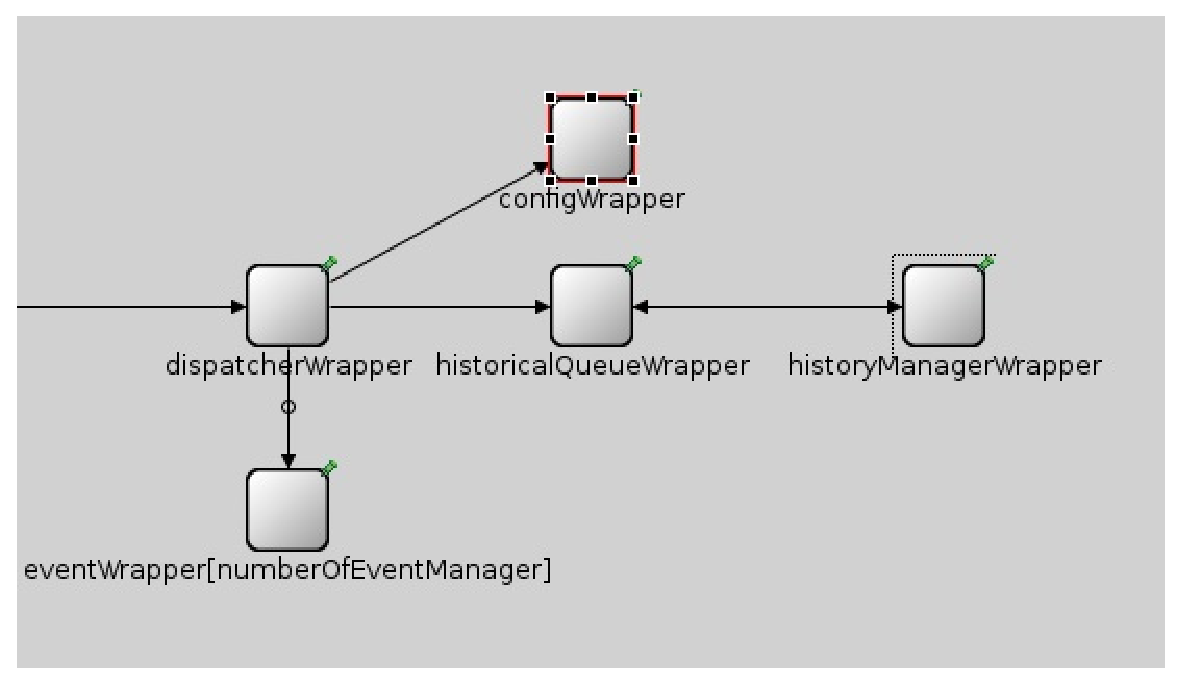
\includegraphics[width=0.9\linewidth]{images/ModularSink}
    \caption{Structure of \emph{ModularSink} showing the implemented wrapper modules and their connections.}
    \label{fig:ModularSink}
\end{figure}

The simulated network consists of the \emph{Generator} instance and a instance specializing \emph{ISink} the underlying module and therefore the tested design is configured via a variable type.
The resulting network for data generation is shown in figure \ref{fig:omnet_example_network}.

\begin{figure}
    \centering
    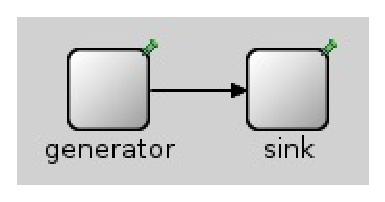
\includegraphics[width=0.3\linewidth]{images/omnet_example_network}
    \caption{Simulated example network showing the \emph{Generator} instance and its connection to the instance of the sink module derived from \emph{ISink}.}
    \label{fig:omnet_example_network}
\end{figure}

\section{Measurement methods}
\label{sec:measurements_methods}
For measuring the performance of the different designs three measurement methods were implemented
Three different methods were implemented for preventing false assumptions based on the result of a single test.
These methods were implemented via different scripts for automated executing and designed dynamically allowing the analyze of various simulations and also either sequential or parallel simulation.

\subsection{Runtime measurement}
\label{sec:measurements_methods_runtime}
The performance of the simulated design can be analyzed by defining a fixed simulation time limit (\emph{sim-time-limit}).
Using the default (non real-time) scheduler this results in a simulation which executes as fast as possible for the required number of events for reaching the simulation time limit.
The required execution time for this simulation represents the performance of the simulation.

Analyzing a parallel simulation using this method does not require special attention, except the handling of multiple resulting runtime values.

\subsection{Processed event count}
\label{sec:measurements_methods_event}
By defining a fixed execution time limit (\emph{cpu-time-limit}) and using the default scheduler the simulation will run for a fixed time.
The number of processed events within this fixed time represents the performance of the simulation.

The simulation of different designs results in contrasting event counts due to the varying number of messages using other designs with more modules and therefore more communication.
For comparison of the performance the created number within a fixed processing time a correction factor must be considered.
This factor describes the ratio of create events using the different designs.
This ratio can be measured using the configuration of the previous method \ref{sec:measurements_methods_runtime} and analyzing the number of created events.

Analyzing a parallel simulation and comparing the performance to a sequential simulation requires further attention to the number of created events.
An additional correction factor is necessary due to the varying number of sent synchronization messages.

\subsection{Real time behavior}
\label{sec:measurements_methods_realtime}
Using the built in real time scheduler \emph{cRealTimeScheduler} the simulation will try to execute the simulation matching the real time.
The performance output (\emph{cmdenv-performance-display}) provides the ratio of simulated seconds per real second.
As described in section \ref{sec:simulation_omnet} this ratio must not differ too much from one for representing a real-time simulation.
The simulated network provides a configurable interval of data generation by \emph{Generator}.
Using a parameter study (described in section \ref{sec:omnet_running_config}) the interval for data generation by \emph{Generator} can be set to values form a range of intervals.
With attention to the performance ratio of the different iterations the interval limit, which still allows real-time simulation, can be determined.

\subsection{Result recording}
The results of the different measurement methods are all extracted from the resulting command line output of the simulation.
The automated test scripts are analyzing the outputs of the executed simulation after finishing the simulation.
For preventing the delay of the measurements and the simulation by writing the output to a file located on an slow peripheral the output files are located on a \emph{ramdisk}.
A \emph{ramdisk} represents a filesystem which is located within the \emph{RAM} (Random access memory) and therefore provides the maximum speed for writing and analyzing outputs.

The implemented test network described in \ref{sec:measurements_network} was developed and analyzed on a Lenovo ideapad U530 with 8GB PC3-12800 DDR3 SDRAM 1600 MHz and a 4th Gen Intel® Core™ i7-4500U (1.8 GHz 200 MHz 4MB) running Kubuntu 15.10.
\cite{lenovo_spec}

\section{Sequential Simulation}
\label{sec:measurements_sequential}
Each of the three developed measurement methods was executed multiple times with the example network.
To eliminate a possible dependency of the resulting performance to the simulated range (e.g. period of simulation time) each method was executed with different times.
The runtime and real-time method was executed for multiple values for the simulation time limit and the event method was executed for different cpu time limits.
This variation of simulation time verifies the testing measurements for independence of the simulated time range and provides reference values for determining correction values for the event method \ref{sec:measurements_methods_event}.

Simulating multiple scenarios three parameter studies (parameter sweeps) were executed for each testing method.

\begin{itemize}
    \item Number of EventManager (default = 1)
    \item Generation interval of \emph{Generator} (default = $100\mu s$)
    \item Polling interval of \emph{HistoryManager} (default = $100\mu s$)
\end{itemize}

During the simulation with different values of a single parameter study the other values are set to the default values.
For the testing scenarios the simulation time limit for the runtime and real-time method or the cpu time limit for the event method was set to one minute.
In the following section the measurement result of the evaluation test (sweep of simulation or cpu time) and the results of the test scenarios are shown and analyzed.

\subsection{Runtime}
\label{sec:measurements_sequential_runtime}

The runtime results of the sequential simulations using both designs and given different simulation time limits are displayed in figure \ref{fig:results_runtime_sim_time}.
The double logarithmic axis shows two linear characteristics for modular and monolithic design.
These nearly parallel linear characteristics show a constant factor in between the runtimes using the two different designs.
The average ratio of runtime using the modular design over the runtime using the monolithic design is $3.393$. %TODO refresh
\\

%TODO check if necessary
% \[\frac{\sum\frac{t_{modular}}{t_{monolithic}}}{N} = 2.84\]

%%% runtime over simulation time %%%
\begin{figure}
    \centering
    \pgfplotsset{
        every axis plot/.append style={very thick}
    }
    \begin{tikzpicture}
        \begin{axis}[
        xmode=log,
        ymode=log,
        ylabel={Runtime $[s]$},
        xlabel={Simulation time $[s]$},
        grid=major,
        legend entries={Modular,Monolithic},
        legend style={at={(0.03,0.97)}, anchor=north west}
        ]
        
        \addplot table {results/runtimeResults.Modular.txt};
        \addplot table {results/runtimeResults.Monolithic.txt};
        \end{axis}
    \end{tikzpicture}    
    \caption{Runtime using different designs over different simulation time limits.}
    \label{fig:results_runtime_sim_time}
\end{figure}

The runtime using different designs with a varying number of \emph{EventManagers} is shown in figure \ref{fig:results_runtime_eventmanager}.
As expected there is no obvious dependency of the resulting runtime to the number of included \emph{EventManagers}.
Due to the fixed simulation time the number of created event stays the same.
The only difference introduced by the increasing number of \emph{EventManagers} is the destination of the event typed data.
The required time for transporting the messages and processing the data is untouched.
The increasing number affects the memory usage of the simulation, which is not analyzed within this design test.
The offset, visible in figure \ref{fig:results_runtime_eventmanager}, in between the different designs is representing the ratio of achieved performance regarding the runtime.
The average of this ratio is $3.342$.
\\

%%% runtime over number of event manager %%%
\begin{figure}
    \centering
    \pgfplotsset{
        every axis plot/.append style={very thick}
    }
    \begin{tikzpicture}
    \begin{axis}[
    xmode=log,
    %ymode=log,
    ylabel={Runtime [s]},
    xlabel={Number of \emph{EventManager}},
    grid=major,
    legend entries={Modular,Monolithic},
    legend style={at={(0.97,0.5)},anchor=east}
    ]
    
    \addplot table {results/time/simtimeEventManagerResults.Modular.txt};
    \addplot table {results/time/simtimeEventManagerResults.Monolithic.txt};
    \end{axis}
    \end{tikzpicture}    
    \caption{Runtime using different designs over variing number of \emph{EventManager}.}
    \label{fig:results_runtime_eventmanager}
\end{figure}

The runtime using different designs with a varying polling interval by the \emph{HistoryManager} is shown in figure \ref{fig:results_runtime_polling}.
These results are again shown in a double logarithmic plot for easier recognition of both plots following a potential characteristic, which is visible as linear plots.
As expected the required runtime is sinking with increasing polling interval.
This behavior can be explained by the sinking frequency of polling operations and thus a decreasing communication.
The offset in between the two plots shown in figure \ref{fig:results_runtime_polling} is, due to the double logarithmic display, representing the ratio in between the runtimes using different designs.
The average ratio of runtime using the modular design over the runtime using the monolithic design is $7.809$.
\\
%%% runtime over polling interval %%%
\begin{figure}
    \centering
    \pgfplotsset{
        every axis plot/.append style={very thick}
    }
    \begin{tikzpicture}
    \begin{axis}[
    xmode=log,
    ymode=log,
    ylabel={Runtime [s]},
    xlabel={Polling interval [ns]},
    grid=major,
    legend entries={Modular,Monolithic},
    legend style={at={(0.97,0.97)}, anchor=north east}
    ]
    
    \addplot table {results/time/simtimePollingResults.Modular.txt};
    \addplot table {results/time/simtimePollingResults.Monolithic.txt};
    \end{axis}
    \end{tikzpicture}    
    \caption{Runtime using different designs over varying polling interval by the \emph{HistoryManager}.}
    \label{fig:results_runtime_polling}
\end{figure}

The runtime using different designs with a varying generation interval by the \emph{Generator} is shown in figure \ref{fig:results_runtime_generation}.
Similar to the previous figure these results are also shown in a double logarithmic plot showing the potential characteristic of sinking required runtime with increasing generation interval.
Again the noticeable offset in between the plots is due to a ratio of resulting runtimes.
The average ratio of runtime using the modular design over the runtime using the monolithic design is $1.588$.
\\

%%% runtime over generation interval %%%
\begin{figure}
    \centering
    \pgfplotsset{
        every axis plot/.append style={very thick}
    }
    \begin{tikzpicture}
    \begin{axis}[
    xmode=log,
    ymode=log,
    ylabel={Runtime [s]},
    xlabel={Generation interval [ns]},
    grid=major,
    legend entries={Modular,Monolithic},
    legend style={at={(0.97,0.97)}, anchor=north east}
    ]
    
    \addplot table {results/time/simtimeGenerationResults.Modular.txt};
    \addplot table {results/time/simtimeGenerationResults.Monolithic.txt};
    \end{axis}
    \end{tikzpicture}    
    \caption{Runtime using different designs over varying generation interval by the \emph{Generator}.}
    \label{fig:results_runtime_generation}
\end{figure}


Analyzing the resulting outputs the ratio of generated messages (events) regarding the different designs can be determined.
The average ratio of number of created events using the modular design over the number of created events using the monolithic design is $2.149$.
This ratio will be used as correction value for the next measurement method analyzing the created events within a fixed cpu time.

\subsection{Created events}
\label{sec:measurements_sequential_event}

The results of testing the simulations and analyzing the number of created events within a given cpu time are displayed in figure \ref{fig:results_event_cpu_time}.
Similar to the previous section a double logarithmic display was used for analyzing the characteristic of the plots.
The courses show potential characteristics and are nearly linear and parallel this leads to the assumption of a constant ratio in between the used designs.
The average ratio of number of created events using the modular design over the number of created event using the monolithic design is $0.284$. %TODO refresh
For comparison to the previous and following test method the reciprocal value is calculated and equals $3.521$.
\\

%TODO check if necessary
%\[\frac{\sum\frac{eventcount_{modular}}{eventcount_{monolithic}}}{N} = 0.549\]

%%% event number over cpu time %%%
\begin{figure}
    \centering
    \pgfplotsset{
        every axis plot/.append style={very thick}
    }
    \begin{tikzpicture}
        \begin{axis}[
        xmode=log,
        ymode=log,
        ylabel={Created event},
        xlabel={Cpu time $[s]$},
        grid=major,
        legend entries={Modular,Monolithic},
        legend style={at={(0.03,0.97)}, anchor=north west}
        ]
        
        \addplot table {results/eventResults.Modular.txt};
        \addplot table {results/eventResults.Monolithic.txt};
        \end{axis}
    \end{tikzpicture}    
    \caption{Created events for different designs over different cpu time limits.}
    \label{fig:results_event_cpu_time}
\end{figure}

The number of created events using different designs and a varying number of \emph{EventManagers} is showed in figure \ref{fig:results_event_eventmanager}.
As expected and similar to the results of the runtime with a varying number of \emph{EventManagers} there is no noticeable dependency of the created events to the number of \emph{EventManagers}.
This presumption was done because by changing the number of instantiated \emph{EventManagers} only the destination of the transmitted events is affected but not the number of events.
Using the double logarithmic visible as offset the ratio in between the different designs is showed in figure \ref{fig:results_event_eventmanager}.
This ratio is defined by the number of created events using a modular design over the number of created events using a monolithic design.
The average of this ratio is $0.273$.
For comparison to the previous and following test method the reciprocal value is calculated which equals $3.663$.
\\

%%% events over Event managers %%%
\begin{figure}
    \centering
    \pgfplotsset{
        every axis plot/.append style={very thick}
    }
    \begin{tikzpicture}
    \begin{axis}[
    xmode=log,
    %ymode=log,
    ylabel={Created events},
    xlabel={Number of EventManager},
    grid=major,
    legend entries={Modular,Monolithic},
    legend style={at={(0.97,0.5)},anchor=east}
    ]
    
    \addplot table {results/event/cputimeEventManagerResults.Modular.txt};
    \addplot table {results/event/cputimeEventManagerResults.Monolithic.txt};
    \end{axis}
    \end{tikzpicture}    
    \caption{Created events using different designs over varying number of \emph{EventManager}.}
    \label{fig:results_event_eventmanager}
\end{figure}

The number of created events using different designs and a varying polling interval by the \emph{HistoryManager} is shown in figure \ref{fig:results_event_polling}.
This result is leading to the assumption of no definable dependency of the number of created events to the polling interval of \emph{HistoryManager}.
The offset in between the plots using different designs is although indicating a ratio representing the performance difference of the used designs.
This ratio is defined by the number of created events using a modular design over the number of created events using a monolithic design.
The average of this ratio results for this test in $0.166$.
For comparison to the previous and following test method the reciprocal value is calculated and equals $6.024$.
\\

%%% events over polling interval %%%
\begin{figure}
    \centering
    \pgfplotsset{
        every axis plot/.append style={very thick}
    }
    \begin{tikzpicture}
    \begin{axis}[
    xmode=log,
    ymode=log,
    ylabel={Created events},
    xlabel={Polling interval [ns]},
    grid=major,
    legend entries={Modular,Monolithic},
    legend style={at={(0.97,0.5)},anchor=east}
    ]
    
    \addplot table {results/event/cputimePollingResults.Modular.txt};
    \addplot table {results/event/cputimePollingResults.Monolithic.txt};
    \end{axis}
    \end{tikzpicture}    
    \caption{Created events using different designs over variing polling interval by the \emph{HistoryManager}.}
    \label{fig:results_event_polling}
\end{figure}

The number of created events using different designs and a varying generation interval by the \emph{Generator} is shown in figure \ref{fig:results_event_generation}.
Similar to the polling interval of \emph{HistoryManager} shown in \ref{fig:results_event_polling} there is no dependency identifiable.
The offset is related to the ratio in between the designs and the average ratio is $0.436$.
For comparison to the previous and following test method the reciprocal value is calculated and equals $2.294$.
\\

%%% events over generation interval %%%
\begin{figure}
    \centering
    \pgfplotsset{
        every axis plot/.append style={very thick}
    }
    \begin{tikzpicture}
    \begin{axis}[
    xmode=log,
    ymode=log,
    ylabel={Created events},
    xlabel={Generation interval [ns]},
    grid=major,
    legend entries={Modular,Monolithic},
    legend style={at={(0.97,0.5)},anchor=east}
    ]
    
    \addplot table {results/event/cputimeGenerationResults.Modular.txt};
    \addplot table {results/event/cputimeGenerationResults.Monolithic.txt};
    \end{axis}
    \end{tikzpicture}    
    \caption{Created events using different designs over variing generation interval by the \emph{Generator}.}
    \label{fig:results_event_generation}
\end{figure}

\subsection{Real-time}
\label{sec:measurements_sequential_realtime}

The real-time results of the sequential simulations using both designs and given different simulation time limits are displayed in figure \ref{fig:results_realtime_sim_time}.
The simulation time limit defines the runtime of a real-time simulation, but does not affect the performance, i.e. the frequency and complexity of calculations.
Therefore the result shows as expected no recognizable dependency of the achievable generation interval to the simulation time.
Although an offset in between the different designs is visible.
This offset represents the ratio of achievable generation interval using a modular design over the achievable generation interval using a monolithic design.
The average of this ratio is $1.717$.\\

% realtime over sim time
\begin{figure}
    \centering
    \pgfplotsset{
        every axis plot/.append style={very thick}
    }
    \begin{tikzpicture}
        \begin{axis}[
        xmode=log,
        ymode=log,
        ylabel={Achievable real time generation interval [ns]},
        xlabel={Simulation time [s]},
        grid=major,
        legend entries={Modular,Monolithic},
        legend style={at={(0.97,0.97)}, anchor=north east}
        ]
        
        \addplot table {results/realTimeResults.Modular.txt};
        \addplot table {results/realTimeResults.Monolithic.txt};
        \end{axis}
    \end{tikzpicture}    
    \caption{Real-time results for different designs over different simulation time limits.}
    \label{fig:results_realtime_sim_time}
\end{figure}

The real-time results for a varying number of \emph{EventManagers} is shown in figure \ref{fig:results_realtime_eventmanager}.
The resulting characteristics show a wide distribution and therefore does not lead to a clear assumption about a to the number of \emph{EventManagers}.
The impact of the different designs is still noticeable.
The average ratio of the achievable generation interval using different designs is $1.488$.
\\

% realtime over event managers
\begin{figure}
    \centering
    \pgfplotsset{
        every axis plot/.append style={very thick}
    }
    \begin{tikzpicture}
    \begin{axis}[
    xmode=log,
    ymode=log,
    ylabel={Achievable real time generation interval [ns]},
    xlabel={Number of \emph{Eventmanagers}},
    grid=major,
    legend entries={Modular,Monolithic},
    legend style={at={(0.97,0.5)}, anchor=east}
    ]
    
    \addplot table {results/realtime/rtEventManagerResults.Modular.txt};
    \addplot table {results/realtime/rtEventManagerResults.Monolithic.txt};
    \end{axis}
    \end{tikzpicture}    
    \caption{Real-time results for different designs over a varying number of \emph{EventManagers}.}
    \label{fig:results_realtime_eventmanager}
\end{figure}

The real-time results for a varying polling interval of \emph{HistoryManager} is shown in figure \ref{fig:results_realtime_polling}.
Similar to the previous results there is no noticeable dependency of the achievable generation interval to the used polling interval.
The performance difference is again shown in the ratio of the achieved intervals.
The average of this ratio is $99999$.
%TODO add average
\\

% realtime over polling interval
\begin{figure}
    \centering
    \pgfplotsset{
        every axis plot/.append style={very thick}
    }
    \begin{tikzpicture}
    \begin{axis}[
    xmode=log,
    ymode=log,
    ylabel={Achievable real time generation interval [ns]},
    xlabel={Polling interval of \emph{HistoryManager} [ns]},
    grid=major,
    legend entries={Modular,Monolithic},
    legend style={at={(0.97,0.5)}, anchor=east}
    ]
    
    \addplot table {results/realtime/rtPollingResults.Modular.txt};
    \addplot table {results/realtime/rtPollingResults.Monolithic.txt};
    \end{axis}
    \end{tikzpicture}    
    \caption{Real-time results for different designs over a varying polling interval of \emph{HistoryManager}.}
    \label{fig:results_realtime_polling}
\end{figure}

The measurement method for analyzing the real-time behavior includes a parameter study of the generation interval of the \emph{Generator}.
Therefore the scenario with varying generation intervals cannot be analyzed using the real-time method.

\subsection{Conclusion of sequential design tests}
\label{sec:measurements_sequential_conclusion}

The analyzed methods were also executed on two additional host machines:

\begin{description}
    \item[Workstation] including an Intel  running Windows 7.
    \item[Build Server] running Linux Mint 17. %TODO????
\end{description}}

Analyzing the results displayed in section \ref{sec:measurements_sequential_runtime}, \ref{sec:measurements_methods_event} and \ref{sec:measurements_methods_realtime} the following insights were made:

\begin{itemize}
    \item Using a modular design the number of events created is bigger, for example the simulated test network resulted in a ratio of created events for a modular design over a monolithic of $9999$. %TODO insert event avg
    \item The increased number of events and the included overhead results in an decreased performance noticeable in each of the three used measurement methods.
    \item The average performance ratio analyzing the runtime is $9999$. %TODO insert runtime avg
    \item The average performance ratio analyzing the real time behavior is $9999$. %TODO insert realtime avg
    \item Varying load simulated by decreased polling interval or generation interval shows a bigger impact on the performance of the modular design network.
\end{itemize}

Using the sequential simulation a monolithic design is recommended for real-time simulations.


\section{Parallel simulation}
\label{sec:measurements_parallel}
The parallel simulation was executed using the \emph{MPI} system openMPI for communication.
The used synchronization method was the \emph{Null Message Protocol} described in section \ref{sec:parallel_omnet_sync}.
A explicit synchronization of the different partitions is necessary due to multiple modules which are using \emph{self-messages} as timers.
The host machine used for developing and executing the simulation provides a 4th Gen Intel® Core™ i7-4500U (1.8 GHz 200 MHz 4MB).
This processor is a dual core CPU supporting hyper threading and therefore provides four logical processors distributed on two physical cores.
The example network includes two autonomous modules which are scheduling their behavior with \emph{self-messages}.
This number of autonomous modules leads to the conclusion for two parallel partitions for parallel simulation.

As described in chapter \ref{cha:parallel_sim} running a simulation distributed on parallel devices requires the mapping of the simulated modules to different parallel partitions.
The first mapping can be applied to both designs and assigns the \emph{Generator} to the partition zero and all modules within the \emph{Sink} to the partition one.
The second tested mapping assigns all modules to the partition zero excepting the \emph{HistoryManager}, which is assigned to the partition one.

As the ratio in between the number of created events by a modular or a monolithic design, described in section \ref{sec:measurements_methods_event}, running a parallel simulation also requires a correction factor due to the varying number of created events by different partitioning.
This dependency is caused by the changing set of transmitted data messages and required synchronization messages.

This correction value can also be determined using the previously discussed method \ref{sec:measurements_methods_runtime}.
The impact of synchronization within parallel simulations is described in section \ref{sec:parallel_omnet_sync}.

\subsection{Runtime}
\label{sec:measurements_parallel_runtime}


\subsection{Event}
\label{sec:measurements_parallel_event}


\subsection{Real-time}
\label{sec:measurements_parallel_realtime}

\subsection{Conclusion of parallel tests}

Considering the results shown in the sections \ref{sec:measurements_parallel_runtime}, \ref{sec:measurements_parallel_event} and \ref{sec:measurements_parallel_realtime} the following insights were made:

\begin{itemize}
    \item The performance of a parallel simulation is depending strongly on the simulated model and its partitioning capabilities.
    \item The used synchronization is highly affecting the achievable performance.
\end{itemize}

\section{Conclusion}
Considering the results of section \ref{sec:measurements_sequential} and \ref{sec:measurements_parallel} the modular design is mostly resulting in a increased number of messages and the caused overhead leads to a debased performance.
Analyzing the simulation of the chosen example network the parallel simulation was not able to achieve an improved performance in comparison to the sequential simulation.
The capabilities of parallel simulation, especially for the usage in the fields of real-time simulation, emulation and \emph{HiL} must be analyzed individually for each simulated model. 
\chapter{openPOWERLINK}
\label{cha:oplk}
openPOWERLINK is an Open Source implementation of the POWERLINK protocol.
The implementation contains the openPOWERLINK stack, different demo applications for various platforms and is designed for an simple introduction into POWERLINK.
The available project should allow manufacturers an easily integration of POWERLINK into their projects.
The Open Source implementation should targets an improved integration an development of new features.

%TODO general description of openPOWERLINK

\section{POWERLINK}
\label{sec:powerlink}
POWERLINK is an industrial real-time communication protocol based on the IEEE 802.3 standard (Ethernet \cite{ethernet_ieee_2016}).
POWERLINK was developed by the members of the Ethernet POWERLINK Standardization Group (\emph{EPSG}).
The \emph{EPSG} consists of different companies located in the field of real time communications, automation and field bus communication. \cite{epsg_hp}

%TODO general description of POWERLINK

\subsection{Network structure}
\label{sec:oplk_powerlink_network}
A POWERLINK network consists of the following two different node types.

\begin{description}
    \item[MN] The managing node exist once within a normal POWERLINK network and controls the communication flow.
    The MN manages all registered network participants, provides a clock and defines the transmission cycle.
    \item[CN] All other nodes within a normal POWERLINK network are controlled nodes and react according to the controls of the \emph{MN}.
\end{description}

Within a POWERLINK network unique POWERLINK addresses (Node IDs) are assigned to each node.
The address range from 1 to 239 is available for all \emph{CNs} and can be assigned freely.
The address 240 is fixed for the \emph{MN}, each node assigned the Node ID 240 automatically performs the \emph{MN} functionalities.
\cite{epsg_epsg_2013}

A simple POWERLINK network consisting of a \emph{MN} connected to one \emph{CN} directly and additional two \emph{CNs} via a Ethernet HUB is shown in figure \ref{fig:powerlink_network}.

\begin{figure}
    \centering
    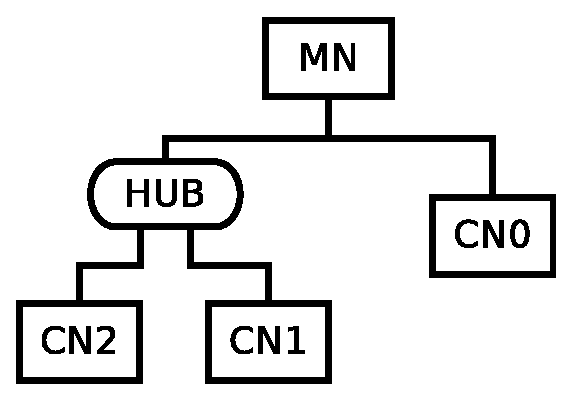
\includegraphics[width=0.5\linewidth]{powerlink_network}
    \caption{POWERLINK network consisting of a \emph{MN} connected to one \emph{CN} and a Ethernet HUB which is connected to two more \emph{CNs}.}
    \label{fig:powerlink_network}
\end{figure}


%TODO describe topologies

\subsection{Frame}
\label{sec:oplk_powerlink_frame}
The POWERLINK frame is embedded in an Ethernet 2 Frames payload and is defined via the Ether type 0x88AB.
Therefore the POWERLINK frame is preceded by the Ethernet 2 Header containing destination \emph{MAC} Address, source \emph{MAC} Address and Ether type.
The payload of an Ethernet 2 Frame can reach up to a length of 1500 bytes succeeding with 4 bytes checksum. \cite[section 3.2]{ethernet_ieee_2016} \cite[section 4.6.1]{epsg_epsg_2013}

In figure \ref{fig:powerlink_frame} the structure of a POWERLINK frame is shown.
The POWERLINK header shown to the left contains the destination and source Node Id preceded by the message type.
The payloads length and content is depending on the transmitted message and thereby defined by the message type. \cite[section 4.6.1.1]{epsg_epsg_2013}

\begin{figure}
    \centering
    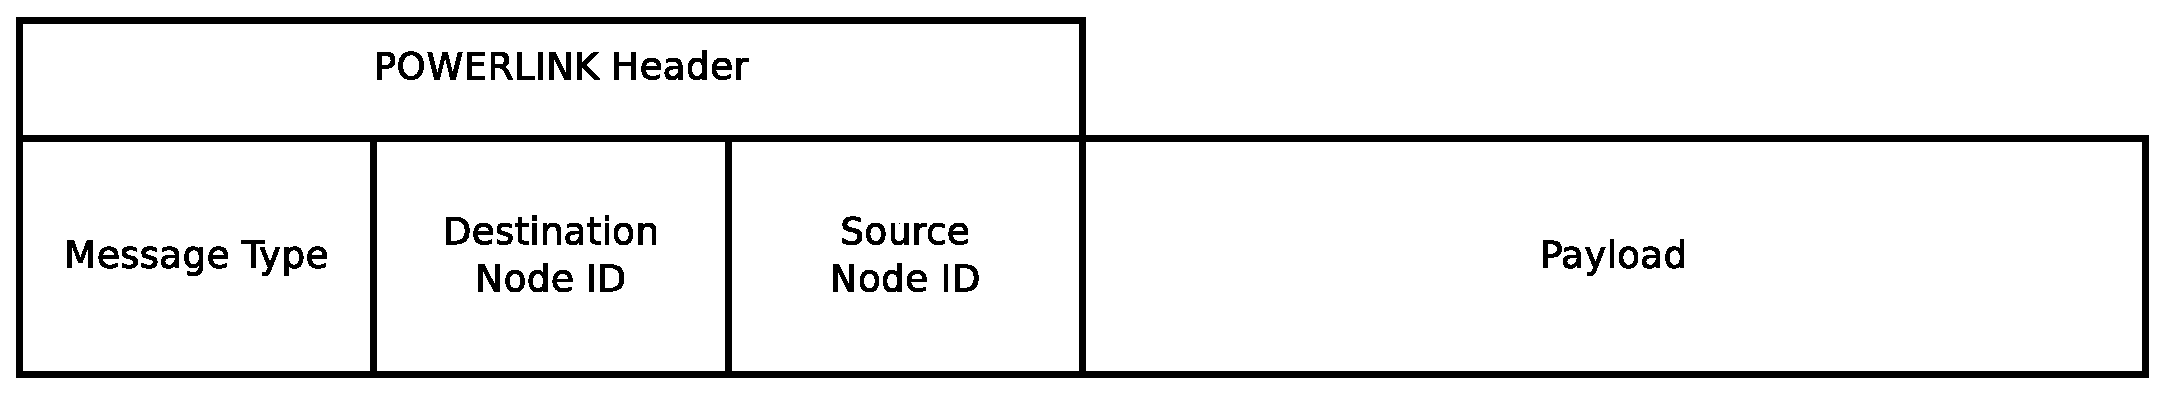
\includegraphics[width=0.9\linewidth]{powerlink_frame}
    \caption{POWERLINK frame showing POWERLINK header and payload.}
    \label{fig:powerlink_frame}
\end{figure}

Detailed information about the different structures of transmitted payloads depending on the message type can be found here \cite[section 4.6.1.1.1]{epsg_epsg_2013}

\subsection{Commands}
\label{sec:oplk_powerlink_commands}

As mentioned above different transmitted POWERLINK messages are defined via the message type.
The following commands are distinguished by the according message type.

\begin{description}
    \item[Soc] Start of cycle is sent by the \emph{MN} as multicast and defines the start of the POWERLINK cycle and the isochronous phase.
    \item[PReq] Poll request is sent by the \emph{MN} to a specific \emph{CN} transmitting data and requesting the transmission data from the \emph{CN}.
    \item[PRes] Poll response is sent by the \emph{CN} as multicast as response to a \emph{PReq} and contains data from the \emph{CN}.
    \item[SoA] Start of Asynchronous is sent by the \emph{MN} as multicast and defines the end of the isochronous phase and the begin of the asynchronous phase.
    \item[ASnd] Asynchronous send is sent either by the \emph{MN} or a \emph{CN} as multicast and contains asynchronous data.
\end{description}

The sequence of sent command within a POWERLINK cycle is shown in the next section.

\subsection{Communication cycle}
\label{sec:oplk_powerlink_commcycle}

The POWERLINK communication cycle is separated in two different phases.

The isochronous phase is the first part of a POWERLINK cycle and is started by the \emph{MN} sending a \emph{SoC} message.
Within this phase the \emph{MN} is polling each \emph{CN} with registered isochronous data.
This polling is accomplished via sending \emph{PReq} message to each \emph{CN}.
This message includes information for the \emph{CN} and also isochronous data which should be sent from the \emph{MN} to the specific \emph{CN}.
After the reception of the \emph{PReq} message the \emph{CN} is sending a \emph{PRes} message as multicast.
This message includes all isochronous data which is requested by the \emph{MN} or any other \emph{CN}.
By multicasting this message each node which should receive a specific data set is immediately receiving the new values. \cite[section 4.2.4.1.1]{epsg_epsg_2013}

When the last isochronous \emph{CN} sent its \emph{PRes} message the isochronous phase is over.
The end of this phase and the start of the asynchronous phase is marked by the sent \emph{SoA} message by the \emph{MN}.
This message contains information about the node which is assigned to the current asynchronous slot.
In each cycle the \emph{MN} assigns the asynchronous slot to either itself or to a \emph{CN}.
Additionally the requested service is transmitted.
Demands a \emph{CN} the assignment to a asynchronous slot this must be communicated to the \emph{MN} either by the \emph{PRes}, \emph{IdentResponse} or \emph{StatusResponse} message.
The communicated number of pending asynchronous messages can additionally provide a priority for better scheduling. \cite[section 4.2.4.1.2]{epsg_epsg_2013}


In figure \ref{fig:powerlink_cycle} a simple POWERLINK communication cycle is shown.
Above the horizontal time axis all command sent by the \emph{MN} are shown.
Commands sent by different \emph{CNs} are displayed below the axis.
This communication cycle shows the isochronous phase marked by the dotted box to the left.
This phase includes the starting command \emph{SoC} and the sequential polling of each \emph{CN}.
This example matches the shown network in figure \ref{fig:powerlink_network} and contains three \emph{CNs}.
The different \emph{CNs} are immediately responding to the polling request.

At the right side in figure \ref{fig:powerlink_cycle} the asynchronous phase is marked by the dashed box.
The asynchronous phase contains the \emph{SoA} command  and following asynchronous data transmission.

\begin{figure}
    \centering
    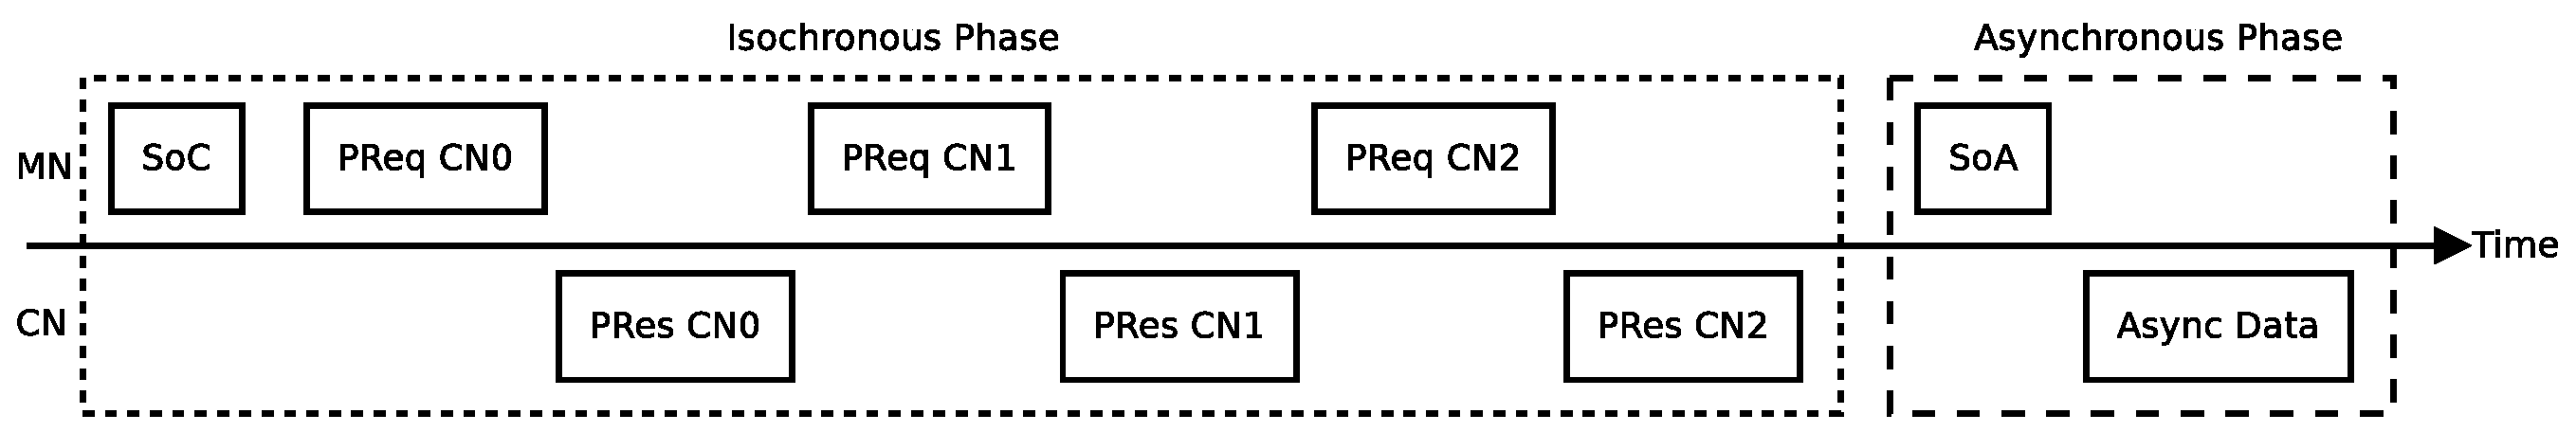
\includegraphics[width=0.95\linewidth]{powerlink_cycle}
    \caption{POWERLINK communication cylce containing Isochronous Phase with polling of three \emph{CNs} and Asynchronous Phase.}
    \label{fig:powerlink_cycle}
\end{figure}

\subsection{Data transmission}
\label{sec:oplk_powerlink_data}


\section{Structure}
\label{sec:oplk_structure}
The openPOWERLINK stack distribution package is structured in different main directories containing demo applications, documentation, driver implementation, the stack sources and multiple more.

For this paper the most important parts are the stack sources and demo applications..
Furthermore an additional simulation directory will be added whose content will be discussed in section \ref{sec:porting_simstub_sim}.

The \emph{apps} folder contains different demo application for embedded targets, linux and windows operating systems.
These demo applications contain exemplary implementations of \emph{MNs} and \emph{CNs}.
These application are analyzed and ported to demo applications within OMNeT++ in the section \ref{sec:porting_demo}.

\subsection{stack folder}
\label{sec:oplk_structure_stack}
The stack folder contains the following structure. \cite{openpowerlink_doc} %TODO: refine citation
\begin{description}
    \item[build] build directory for output files of the build process.
    \item[cmake] configuration files for the build toolchain.
    \item[include/oplk] represents the main include directories for all applications using the openPOWERLINK stack.
    \item[include/common] represents a common internal include directory.
    \item[include/kernel] represents an internal include directory for kernel modules.
    \item[include/target] represents an internal include directory with target specific files.
    \item[include/user] represents an internal include directory for user modules.
    \item[lib] represents the installation directory for the openPOWERLINK libraries.
    \item[proj] represents the directory containing different library projects.
    \item[src/arch] represents a source directory with architecture specific functions.
    \item[src/common] represents a source directory with sources for user and kernel layer.
    \item[src/user] represents a source directory with sources for the user layer.
    \item[src/kernel] represents a source directory with sources for the kernel layer.
\end{description}

This structure represents the architecture of the openPOWERLINK stack, which is explained in the following section.

\subsection{Architecture}
\label{sec:oplk_structure_architecture}

The openPOWERLINK stack is generally separated in kernel and user layer.
This separation was introduced with the version 2.X of the openPOWERLINK stack and is detaching the higher level user functionalities from the lower level kernel functions including time critical behavior and hardware access.

The user and kernel layer are separated by the communication abstraction layer (\emph{CAL}).

%TODO explain architecture including user, kernel, CAL, AMI, HAL, ...
%TODO figure with system overview

\subsection{Configuration and build}
\label{sec:oplk_structure_build}

%TODO rework
The build tool \emph{CMAKE} is used for dynamic creation of according makefiles using definitions and special sources for platform dependency.

Within the openPOWERLINK folder structure the main \emph{CMAKE} file \emph{CMakeLists.txt} checks the current \emph{CMAKE\_SYSTEM\_NAME} variable and creates the according makefile.
The subfolder cmake the general and platform specific cmake-files are located.
The general files \emph{directories.cmake} and \emph{stackfiles.cmake} are always included in the generation process.

Within \emph{directories.cmake} the location of the source, include, user-, kernel-space, architecture files are defined.
The \emph{stackfiles.cmake} file contains the definitions for specific source files grouped in categories like \emph{event}, \emph{cal} and many more.
The platform specific source files are also defined within this file with the according names.

The global \emph{CMAKE} file loads according to the \emph{CMAKE\_SYSTEM\_NAME} and \emph{CMAKE\_SYSTEM\_PROCESSOR} variable the correct system specific options file.
This option file includes options for enabling and disabling part of the openPOWERLINK stack.
For example the generation of the \emph{CN} or \emph{MN} library can be en- or disabled.
Further options are platform specific and provide configuration possibilities for specific usages.

Checking the defined options the according projects are included in the generation and later on the build process.
These projects are located in the \emph{proj} folder.


\subsection{\emph{Proj} folder} %TODO check is useful
\label{sec:oplk_structure_proj}
The \emph{proj} folder contains different directories for three target systems:

\begin{description}
    \item[generic] contains projects for embedded targets without underlying operating systems.
    Providing implementations of \emph{MN} and \emph{CN} for different targets.
    \item[linux] contains projects for linux operating systems using different technologies (Kernel Module, dirver, ...).
    \item[windows] contains projects for windows operating systems using different technologies (Kernel Module, dirver, ...).
\end{description}

Within a specific target folder the different projects are located.
For example the projects \emph{liboplkmn} and \emph{liboplkcn} exist for windows and linux systems.
The different projects represent either different functionalities or different targets and included technologies.

Specific files for each project are located in each folder, including a \emph{CMakeListst.txt} file.
This is included by the according option files.
Within these \emph{CMakeListst.txt} file the specific source files are gathered and set within variables like \emph{LIB\_SOURCES}.
These variables are used for defining the build targets.
The type, location and additional libraries are also either defined within the project files or the option files.

The build targets mostly are libraries which can be linked to the resulting application.

\section{Platform dependency}
\label{sec:oplk_platform}
%TODO: rework and enhance
As described in section \ref{sec:oplk_structure} the configuration and build process defines the according platform specific implementations and libraries.

For platform specific functionalities the implementation of the openPOWERLINK stack uses common header files with specific implementations.

For defining which implementations are platform specific the \emph{CMAKE} file \emph{stackfile.cmake} is analyzed.

The following modules are implemented platform dependent:

\begin{description}
    \item[oplkinc.h] provides macros for target specific functions which depends on the targeting platform or operating systems.
    Defined are small standard functions regarding memory operations.
    \item[Trace] module providing a function for tracing the execution.
    \item[\emph{OBD} configuration] containing specific for functions for storing and restoring of the \emph{OD}.
    The implementation is split in functions regarding file operations and a generic cyclic redundancy check (\emph{CRC}) calculation.
    \item[\emph{SDO} via \emph{UDP}] this implementation contains the transmission of \emph{SDO}s via user datagram protocol (\emph{UDP}).
    The specific implementations provide usage of operating system calls of linux and windows or the usage of a generic header \emph{socketwrapper.h} which allows the implementation for other targets.
    \item[\emph{CAL}] includes different interfaces for the user and kernel space for each containing module (control, \emph{DLL}, \emph{PDO}, error handler, event).
    \item[Timer] providing functions for setting timer.
    \item[Circular buffer] providing the system specific functionalities used within the \emph{circular\_buffer} as creation, allocation, deallocation, locking, connecting and disconnecting.
    \item[Memmap] providing an interface for the memory mapping library used for memory mapped communication in between kernel and user space.
    \item[Target] providing an interface for target specific functions as sleep, interrupt control, tick and implementations of locks and mutexes.
    \item[\emph{AMI}] providing an interface for architecture specific memory functions.
    \item[Edrv] represents the Ethernet driver which is communicating with the used Ethernet media access control (\emph{MAC}) controller.
\end{description}

The porting ot the described platform dependencies to the OMNeT++ simulation environment and the according analyzes are described in the following chapter.
\chapter{Simulation of openPOWERLINK}
\label{cha:porting}
The development of an OMNeT++ simulation including a POWERLINK network consisting of multiple nodes is achieved by porting the openPOWERLINK stack to the OMNeT++ environment.

For developing a simulation embedding an openPOWERLINK node, the stack must be ported within the OMNeT++ environment.
Therefore the platform dependencies as discussed in section \ref{sec:oplk_platform} are analyzed and additional simulation specific implementations are introduced.

The design measurement shown in chapter \ref{cha:measurements} resulted in the recommendation for a monolithic design for improved performance.
Using this recommendation the platform dependencies shown in section \ref{sec:oplk_platform} are analyzed and different library projects are compared.
The result is the most monolithic stack configuration with the demand for the following modules to be implemented in the simulation stub.

\begin{itemize}
    \item edrv
    \item hrestimer
    \item target
    \item sdoudp
\end{itemize}

Additionally to the essential modules above the \emph{trace} module was also implemented for forwarding additional trace informations to the simulation environment.

For showing the implementations and giving examples of the strategies and implementations the Ethernet driver module \emph{edrv} was chosen.

The intention is to separate the simulation specific implementations and changes within the openPOWERLINK stack and the OMNeT++ implementations providing the simulation environment.
This is achieved by the introduction of a simulation stub in the openPOWERLINK stack.

\section{Simulation stub}
\label{sec:porting_simstub}

The simulation stub should provide the same functions and signatures for the usage within the openPOWERLINK stack but should forward according function calls to the external simulation environment.

For minimizing the in the openPOWERLINK stack introduced functionalities the simulation stub is separated into two components the specific implementations for the \emph{sim} target and the simulation interface.
Both are explained in the following sections.

\subsection{Target specific implementation}
\label{sec:porting_simstub_target}

Similar to the specific implementations for various modules in the openPOWERLINK stack (as described in section \ref{sec:oplk_architecture}) the  dependent implementation for the \emph{sim} target were added.

Those implemented functions contain mostly simple calls to the according function of the simulation interface.
The appendix section \ref{app:simulation_edrv_target} shows the implementation of the \emph{edrv\_sendTxBuffer} function from the \emph{edrv} implementation for the \emph{sim} target.
The implementation simply consists of a function call of the according function of the simulation interface.

Within the simulation target specific implementations of different modules only function calls to the simulation interface and small parameter conversions are implemented.
This simulation interface is located in a new folder named \emph{sim}.
The content of this folder and the targeted purpose is shown in the next section.

\subsection{Simulation interface}
\label{sec:porting_simstub_siminterface}
The \emph{sim} folder contains two main folders separating the source and include files.
Each module within the openPOWERLINK stack which should be connected to the simulation environment has its specific simulation module within the simulation interface.
The naming of the different simulation interface modules contains the common prefix \emph{sim} separated with a hyphen from the implemented module.

The following list shows the added files for connecting the \emph{edrv} module to the simulation environment.

\begin{description}
    \item[stack/kernel/edrv/edrv-sim.c] Target specific implementation of the \emph{edrv} module.
    \item[sim/include/sim-edrv.h] Header file of simulation interface for the \emph{edrv} module.
    \item[sim/src/sim-edrv.c] Implementation of simulation interface for the \emph{edrv} module.
\end{description}

\begin{sloppypar}
The simulation interface contains all functions which are used by the ported stack module.
Additionally each simulation interface provides a set\emph{ModuleName}Functions function.
For all functions which should be connected to the simulation the according types are defined as typedefs and grouped in a global structure named t\emph{ModuleName}Functions.
For a common include file containing all types required for the simulation interface the typedefs for each function pointer and the structures are defined within the header file \emph{sim.h}.
Such a struct is passed to the set\emph{ModuleName}Functions function.
This function is checking each containing function pointer and only when all of them are valid the structure is saved in the static instance and a flag is set for valid initialization.
\end{sloppypar}

When a function of the simulation interface is called by the stack the static instance is checked and when the functions were initialized correctly the according function is called.
Therefore the external defined functions, passed by a struct of function pointers, are called and the connection from the stack to the simulation environment is established.

For configuring the simulation interface from the simulation environment the accessible function set\emph{ModuleName}Functions is declared as exported function for shared libraries.
This is done via the preprocessor macro \emph{OPLKDLLEXPORT} defined by the openPOWERLINK stack.
This macro is defined within the target specific includes located in \emph{stack/include/oplk/targetdefs} as described in section \ref{sec:oplk_platform_hardware}.

The appendix section \ref{app:simulation_edrv} shows the definition and implementation of the simulation interface module \emph{edrv} regarding the initialization and the sendTxBuffer function as example.
As shown in the appendix an additional parameter was added to each function.
This is necessary for supporting the simulation of multiple openPOWERLINK stack instances within a single simulation.
The used strategy is described in section \ref{sec:porting_stack_multiinstance}.

For the opposite direction of calling a stack function from the simulation environment two cases are distinguished.

\begin{enumerate}
    \item Is the desired function already an exported function and e.g. part of the public \emph{API} it is resolved and called directly from the simulation environment.
    \item Is the desired function not exported and the export of this function is not allowed, or the signature should not be changed a according simulation interface module must be inserted.
    This module is similar to the other simulation interface module located in the simulation folder and exports all accessible functions.
    Within the implementation of these functions the according stack function can be called directly.
\end{enumerate}

In both cases no simulation stub is required, because no specific implementation is replaced by the simulation, only specific functions are exported.

The communication from the openPOWERLINK stack into the simulation environment and the opposite direction are established.
This connection to the simulation environment is designed independent of OMNeT++ and does not require and OMNeT++ functionalities.
This independence was established for supporting various simulation environments and systems.
The simulation interface can be used with every application and simulation environment which is capable of handling with a native shared library.

For this paper the simulation environment OMNeT++ was chosen and the modified openPOWERLINK stack is embedded in an OMNeT++ simulation.
The following sections show the implementation of the simulation and its different components.

\section{Simulated stack}
\label{sec:porting_stack}
The simulated stack consists of the five implemented modules \emph{edrv}, \emph{hrestimer}, \emph{target}, \emph{sdoudp} and \emph{trace}.
These modules will also be implemented separately within the simulation for representing the simulated structure and functional units.

The result of the successful build process of the modified openPOWERLINK stack is a shared library exporting the by default exported functions and new functions for interacting with the simulation interface.
The structure of the developed simulation and the enclosed components are described in the following section.

\subsection{Simulation structure}
\label{sec:porting_stack_simstructure}
Within the openPOWERLINK simulation the essential folder structure was recommended by OMNeT++ and separates the simulation configuration (\emph{simulations} folder) from the implemented model (\emph{src} folder).
For better representation of custom openPOWERLINK nodes contains the \emph{images} folder icons with an embedded openPOWERLINK logo.

The implemented model within the \emph{src} folder is separated in different folders for the \emph{MN}, the \emph{CN} and a generic node implementation.
These nodes and the implemented hierarchy is described in the section \ref{sec:porting_nodes}.

Approaching the counterpart to the above described simulation interface the generic node contains an \emph{stack/interface} folder containing the implementation of the interface to the simulated openPOWERLINK stack.
The functionalities and the underlying strategy of this interface implementation is described in the following section.

\subsection{Interface Implementation}
\label{sec:porting_stack_interface}
The implementation of the interface within the simulation is based on the following two classes providing the basic functionalities for handling the connection to the simulated stack.

\emph{OplkBase} represents a base class for every interface module connected to the simulated openPOWERLINK stack.
It is implemented as a template class taking a template type for a module.
This module is grouped together with an instance of the second class \emph{SharedLibraryHelper}.

The class \emph{SharedLibraryHelper} is implemented independently of the OMNeT++ framework and provides methods for the handling of an shared library.
The internal implementations are depending on preprocessor macros implemented for Linux and Windows.
Basically the \emph{SharedLibraryHelper} allows the loading of a defined shared library object and the resolving of defined functions.
The shared library is opened during creation of an \emph{SharedLibraryHelper} and is closed during destruction and thereby follows the design principle of Resource Acquisition Is Initialization (RAII).
This ensures the correct closing of all opened shared libraries during shutdown and prevent possible resource leaks.
The resolved functions are returned as std::function objects with the requested types.
The usage of functional objects over simple function pointer allows more dynamic handling within the object oriented environment.

The class \emph{OplkBase} provides a \emph{initModule} method taking an instance of the template type as parameter.
This function creates a new instance of \emph{SharedLibraryHelper} with the internally saved library name and stores the helper object together with the given module in an internal container.

After this creation the helper object and the index of the currently added instances within the internal container is passed to the method \emph{setFunctions}.
This method is defined pure virtual and demands the implementation by a derived class.

Via deriving from \emph{OplkBase} all implemented interface classes contains the functionality of holding the according \emph{SharedLibraryHelper} with an instance of a type than can be defined.
These derived classes are named according to the implemented module with \emph{Oplk} as prefix and located within the interface folder and interface C++ namespace.
The template parameter should usually be defined to a pointer to the according OMNeT++ module which is named simple by the implemented module, e.g. \emph{Edrv} represents the OMNeT++ module for Ethernet driver module.

This connection of \emph{SharedLibraryHelper} and module instance is demanded by the requirement for multiple simulated instance of the openPOWERLINK stack within a single simulation.
This requirement, its consequences, the solution and the implementation are described in the next section.

\subsection{Multiple instances}
\label{sec:porting_stack_multiinstance}
The openPOWERLINK stack is designed as pure ANSI C implementation structured in multiple modules.
The designated usage of the openPOWERLINK stack is the execution on a devices representing each a single node.
For various applications implemented using openPOWERLINK there was no demand on the support for multiple instances on a single system.
Because of this designated usage and no demands for multiple instance the informations about various states, buffer and all other data stored within the openPOWERLINK stack are store in static variables.
These variables exist once in the whole compiled application.
Therefore the simulation of multiple instances within a single application by normal linking of the shared library is not possible.

The solution for this problem was the loading of multiple versions of the same shared library into the memory.
Linux supports the loading of a single shared library multiple times into the memory and therefore creating multiple instances of and static object within the library.
OMNeT++ is supporting Windows and Linux in the same way and for achieving a simulation which is usable in the identical way on either Linux or Windows another strategy was found.

When the binary file of a shared library is copied and named differently both files can be loaded into the memory as different libraries.
This strategy does not require any special functionality and can be implemented for Windows and Linux in the same way.
This handling of multiple shared libraries and the copying of the binary file if demanded is implemented within the \emph{SharedLibraryHelper}.
During creation of a \emph{SharedLibraryHelper} a maximum number of instances can be defined.
Starting with the manually created instance any further instances can be accessed by the method \emph{getNextLibrary} which copies the shared library if necessary and creates a new instance with the copied version.
When a new instance is requested but the maximum number of allowed instances is exceeded an exception is thrown.
When not caught otherwise this exception would cause the simulation to shutdown and the error shown to the user.

As mentioned in section \ref{sec:porting_simstub_siminterface} and shown in appendix section \ref{app:simulation_edrv} the simulation interface includes an instance handle parameter.
This handle is passed when the set\emph{ModuleName}Functions function of an interface module is called and is stored int the static instance information of the the interface module.
When a function call from the openPOWERLINK stack is forwarded to the simulation interface the stored handle is passed to the stored function pointers.
The counterpart within the simulation interface can then assign the function call to a specific instance.
This assignment is done within the derived classes of \emph{OplkBase}.
The derived classes must be implemented as singleton and therefore support only a single instance within the application.
This instance holds the container of modules (given via the method \emph{initModule} and assigned \emph{SharedLibraryHelper} instances.
The passed instance handle represents the index within this internal container and is created after inserting the instances within the \emph{initModule} method of \emph{OplkBase}.

The above mentioned pure virtual method \emph{setFunctions} must be implemented by a derived class and gets the \emph{SharedLibraryHelper} instance and the instance handle (index within internal container) passed by the base class implementation.
Within this method each derived class must initialize the instance of the shared library.
This is done by creating an according structure of function pointers, which can be realized via static methods.
After successful resolving of the set\emph{ModuleName}Functions function this structure with the newly created handle is passed and the according simulation interface is initialized.

When a function call is forwarded from the openPOWERLINK stack over the simulation interface to the static method the stored instance handle is passed as parameter.
This handle can be used for getting the according module instance from the internal container of modules and \emph{SharedLibraryHelper} instances inherited from \emph{OplkBase}.
Using this module instance the according method can be called and the function call is forwarded to the correct instance of a module.

For the opposite direction of communication the \emph{setFunctions} method can be used for resolving the required functions from the according shared library instance and saving them in the given module instance.
When calling one of this resolved function the according shared library instance is used due to the correct saved function.

An overview of this hierarchy and the connections of different instances is shown by an exemplary composition in figure \ref{fig:simulation_instances}
The shown example includes the OMNeT++ environment an the bottom containing two instantiated nodes.
The \emph{MN} and the \emph{CN} represent separate simulated nodes within an POWERLINK network.
Each node contains an \emph{edrv} instance which is registered as module within in the \emph{oplkEdrv} instance.
Above the OMNeT++ environment tow openPOWERLINK stacks are shown, which exists independently of each other.
Each openPOWERLINK stack contains the simulation interface module \emph{sim-edrv} and the target specific implementation \emph{edrv-sim}.
The tow stacks connected to the tow nodes demonstrate the two directions of function calls.

The left side including the \emph{MN} is called by the openPOWERLINK stack forwarding the function call from the \emph{edrv-sim} to the simulation interface \emph{sim-edrv}.
This adds the internal stored handle to the parameters and calls the saved static method of \emph{oplkEdrv}.
Using the passed handle the according save module instance \emph{edrv 0} is accessed and the according function is called.
The shown dashed arrows mark the path of the according return value.

The right side including the \emph{CN} requests the function object for a specific function of \emph{sim-edrv} within stack 1.
The \emph{SharedLibraryHelper} instance saved in \emph{oplkEdrv} returns the correct function object.
This is called by \emph{edrv 1} and therefore the function of \emph{sim-edrv} is directly invoked.
This call is then forwarded to the openPOWERLINK stack directly within \emph{sim-edrv}.

\begin{figure}
    \centering
    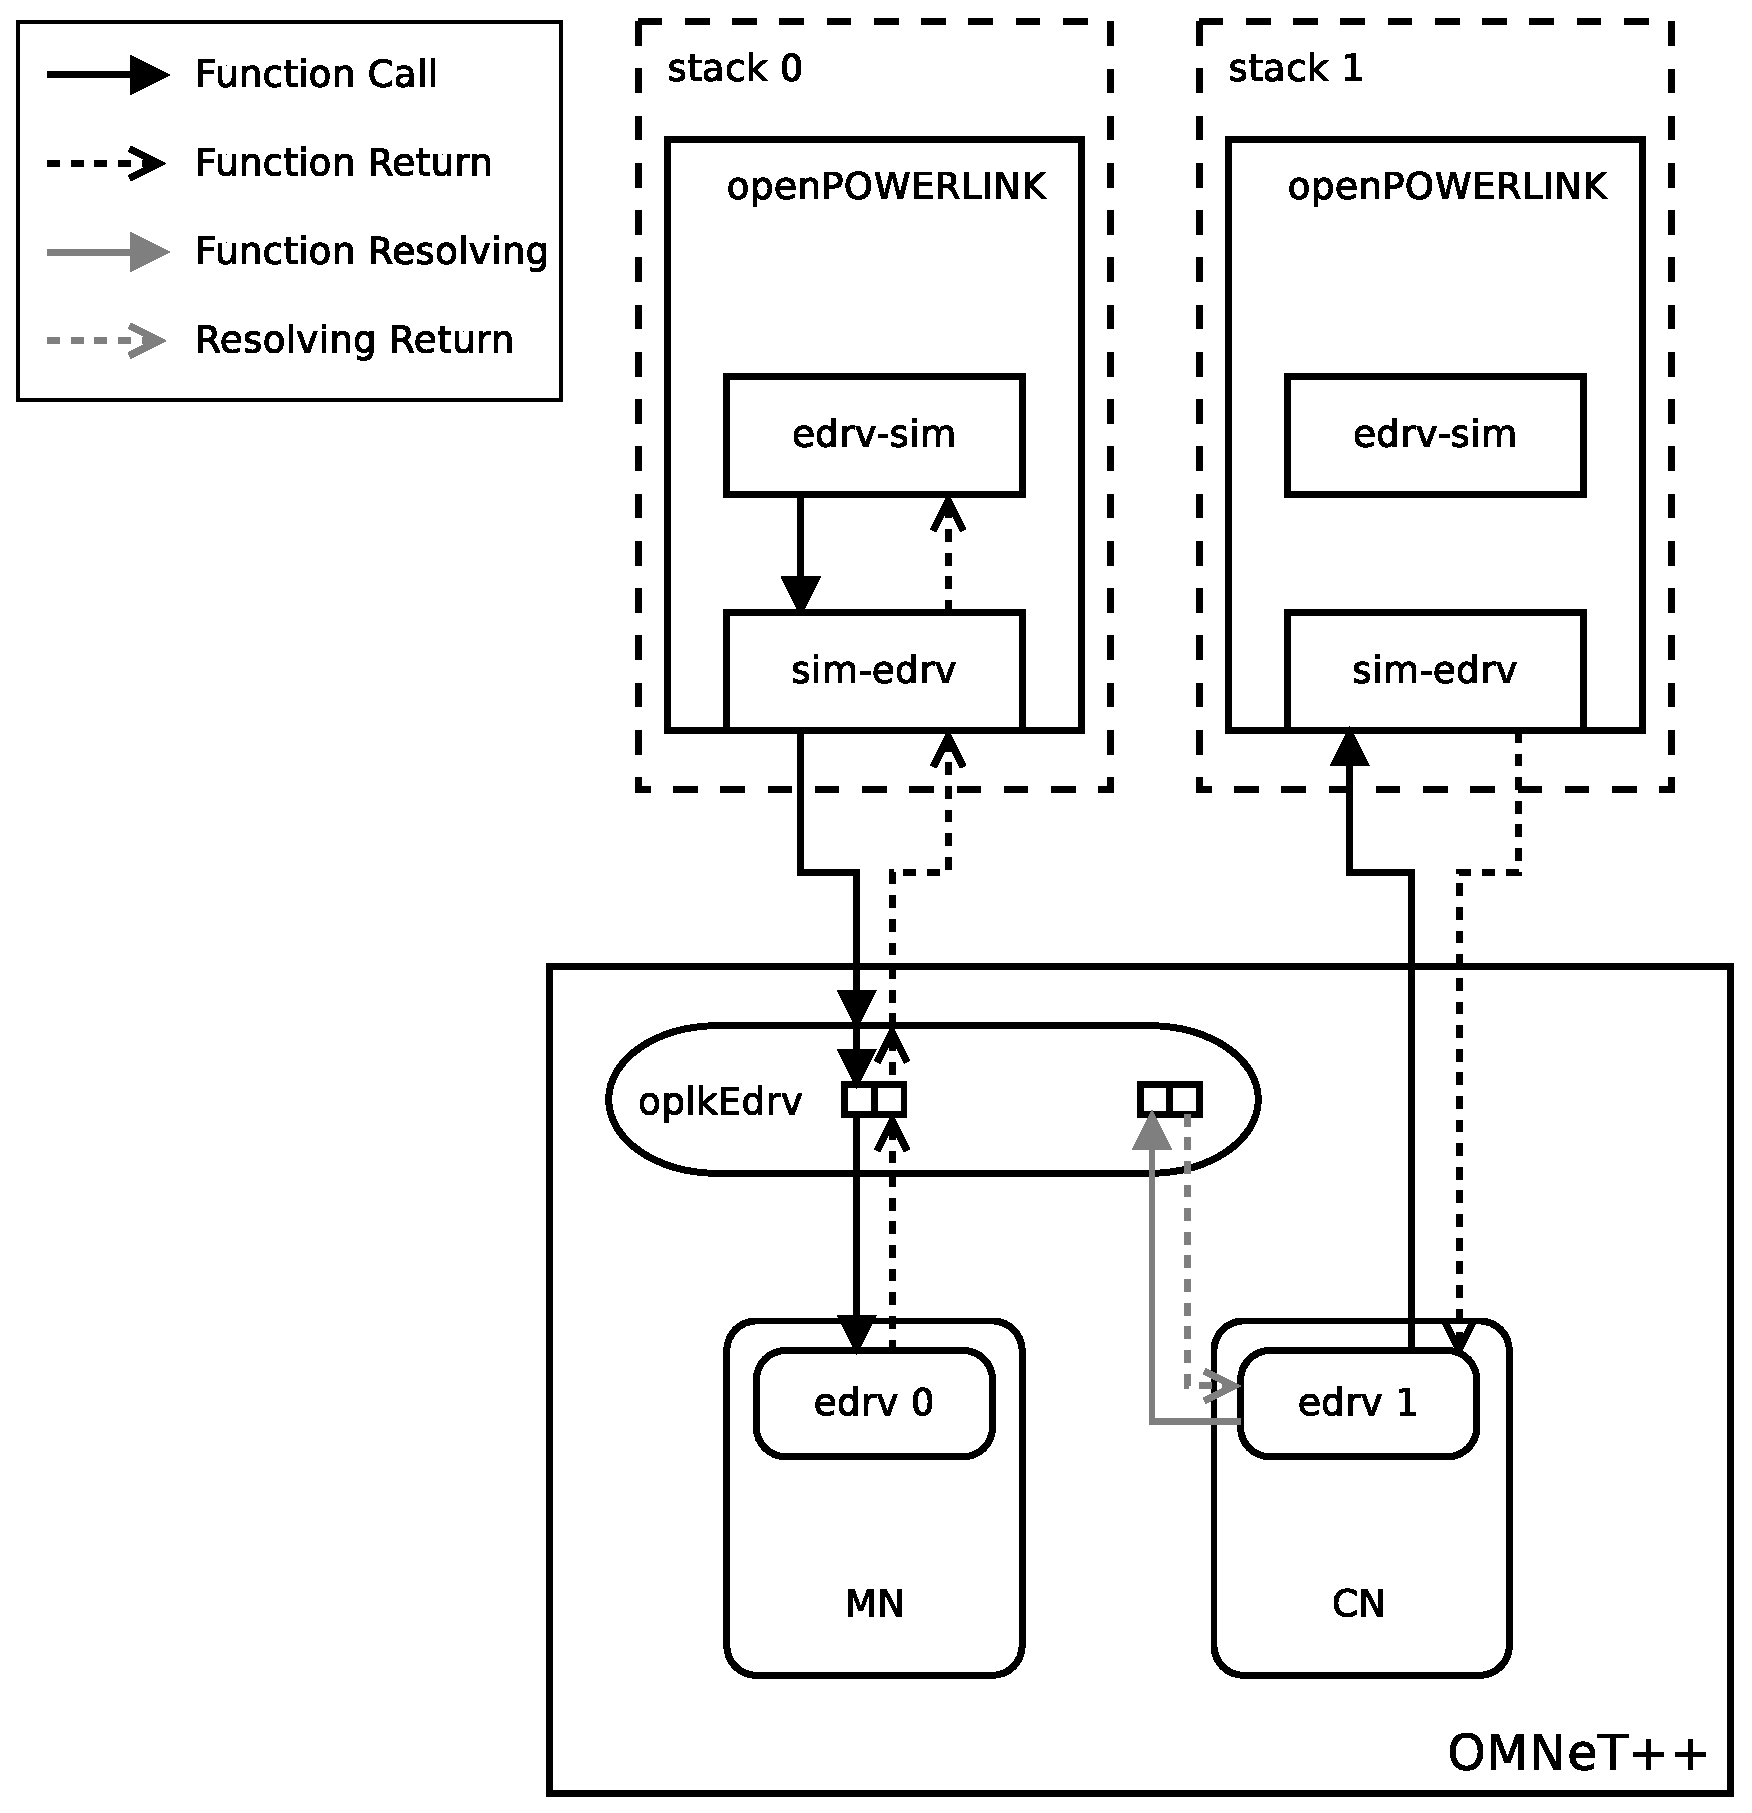
\includegraphics[width=0.7\linewidth]{simulation_instances}
    \caption{Hierarchical overview of the simulation environment, embedded modules the stack interface and simulation interface.}
    \label{fig:simulation_instances}
\end{figure}

The implementation of \emph{OplkBase}, \emph{SharedLibraryHelper} and \emph{OplkEdrv} are shown in appendix section \ref{app:simulation_stackif}.

The further implementation and structuring of the according OMNeT++ modules is described in the following section.

\subsection{Stack module}
\label{sec:porting_stack_stackmodule}

The previous mentioned OMNeT++ modules representing components within the openPOWERLINK stack and invoked by a derived class of \emph{OplkBase} are located in the \emph{stack} folder.
These modules provide the functions which implement the required functionalities for the openPOWERLINK stack.
The combination of these modules illustrate a single openPOWERLINK stack module and represent a single openPOWERLINK stack instance.

\begin{figure}
    \centering
    %TODO make screenshot and embedd
    %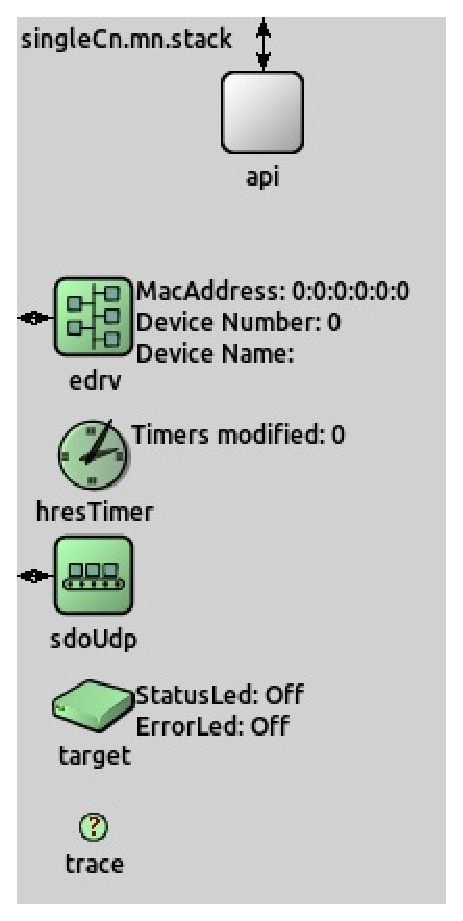
\includegraphics[width=0.7\linewidth]{simulation_stack_module}
    \caption{Composition of compound module representing the openPOWERLINK stack.}
    \label{fig:simulation_stack_module}
\end{figure}


\section{Simulated nodes}
\label{sec:porting_nodes}
%TODO explain different types of nodes

\subsection{Generic node}
\label{sec:porting_nodes_generic}
%TODO explain hierarchy and components of generic node with demo, app and event

\subsection{MN}
\label{sec:porting_nodes_mn}
%TODO explain special properties of MN

\subsection{CN}
\label{sec:porting_nodes_cn}
%TODO explain special properties of CN

%As described in section \ref{sec:oplk_platform} multiple modules contain platform specific functionalities.
%The openPOWERLINK stack can be built with various configurations, depending on the settings and the compositions configured individually more or less platform specific modules are used.
%These configurations are defined within the different projects in the \emph{proj} folder, as explained in section \ref{sec:oplk_structure_proj}.
%
%\section{Analyze of existing projects}
%\label{sec:porting_projects}
%
%\subsection{liboplkmn}
%\label{sec:porting_projects_liboplkmn}
%
%The \emph{liboplkmn} represents a \emph{MN} library consisting of a single library including the user and kernel space.
%Analyzing the \emph{liboplkmn} for linux results in following modules which must be ported:
%
%\begin{itemize}
%    \item Target
%    \item Timer
%    \item Edrv
%    \item \emph{SDO} via \emph{UDP}
%    \item Trace
%\end{itemize}
%
%The first step for the implementation of the \emph{MN} library for OMNeT++ is the integration in the configuration and build process within the openPOWERLINK stack.
%Therefore an according options file and toolchain file for integration in the \emph{CMAKE} process are created.


\chapter{Conclusion}
\label{cha:conclusion}

%TODO: rewrite conclusion

% imported from paper
OMNeT++ provides many different features for developing various simulations.
The built in mechanisms for real time simulations represent a possibility for emulations and the field of \emph{HiL}.
Due to the simulated system's effect on the achievable capabilities, each system must be analyzed individually.
Such an analyze can also be used for the implementation of an optimized scheduler which can lead to improved performances for specific applications.


The general increased overhead of a modular design can limit the achievable timings of a real time simulation, but executed with parallelization this can lead to a improved performance.
Is the efficient parallel execution of a simulated system not possible due to a too high level of dependencies between modules a monolithic design should be considered for decreasing simulation overhead


The open source project OMNeT++ provides the possibility of analyzing the simulation and developing optimized and customized solutions.
These solutions provide remarkable opportunities for emulation and the field of \emph{HiL} and are therefore useful for different applications.

%%%----------------------------------------------------------
%%%Anhang
\appendix
\chapter{OMNeT++ Code Snippets}
\label{app:omnetpp_code}

\section{cRealTimeScheduler}
\label{app:omnetpp_code_real_time_scheduler}

\lstinputlisting[caption=Definition of \emph{cRealTimeScheduler},firstnumber=138,firstline=138,lastline=200]{\omnetpproot/include/cscheduler.h}
\lstinputlisting[caption=Implementation of \emph{cRealTimeScheduler},firstnumber=63,firstline=63,lastline=133]{\omnetpproot/src/sim/cscheduler.cc}

\section{sockets Sample}
\label{app:omnetpp_code_socket}


\subsection{SocketRTScheduler}
\label{app:omnetpp_code_socket_scheduler}

\lstinputlisting[caption=Definition of \emph{SocketRTScheduler}]{\omnetpproot/samples/sockets/SocketRTScheduler.h}
\lstinputlisting[caption=Implementation of \emph{SocketRTScheduler}]{\omnetpproot/samples/sockets/SocketRTScheduler.cc}

\subsection{ExtHttpClient}
\label{app:omnetpp_code_socket_http}

\lstinputlisting[caption=Implementation of \emph{ExtHttpClient}]{\omnetpproot/samples/sockets/ExtHttpClient.cc}

\subsection{ExtTelnetClient}
\label{app:omnetpp_code_socket_telnet}

\lstinputlisting[caption=Implementation of \emph{ExtTelnetClient}]{\omnetpproot/samples/sockets/ExtTelnetClient.cc}


% placement settings for following figures
%\floatplacement{figure}{H}

\chapter{Further design Measurements}
\label{app:measurements}

This chapter includes all plots of analyzed design measurements executed on the additional host machines.

\section{Workstation measurements}
\label{app:measurements_workstation}

\subsection{Runtime}
\label{app:measurements_workstation_runtime}

% runtime over simtime
\begin{figure} [H]
    \centering
    \pgfplotsset{
        every axis plot/.append style={very thick}
    }
    \begin{tikzpicture}
    \begin{axis}[
    xmode=log,
    ymode=log,
    ylabel={Runtime [s]},
    xlabel={Simulation time [s]},
    grid=major,
    legend entries={Modular,Monolithic},
    legend style={at={(0.03,0.97)}, anchor=north west}
    ]
    
    \addplot table {../results/workstation/runtimeResults.Modular.txt};
    \addplot table {../results/workstation/runtimeResults.Monolithic.txt};
    \end{axis}
    \end{tikzpicture}    
    \caption{Runtime results for different designs over a varying simulation time.}
    \label{fig:app_workstation_runtime_simtime}
\end{figure}

%%% runtime over number of event manager %%%
\begin{figure} [H]
    \centering
    \pgfplotsset{
        every axis plot/.append style={very thick}
    }
    \begin{tikzpicture}
    \begin{axis}[
    xmode=log,
    %ymode=log,
    ylabel={Runtime [s]},
    xlabel={Number of \emph{EventManager}},
    grid=major,
    legend entries={Modular,Monolithic},
    legend style={at={(0.97,0.5)},anchor=east}
    ]
    
    \addplot table {../results/workstation/runtime/simtimeEventManagerResults.Modular.txt};
    \addplot table {../results/workstation/runtime/simtimeEventManagerResults.Monolithic.txt};
    \end{axis}
    \end{tikzpicture}    
    \caption{Runtime using different designs over variing number of \emph{EventManager}.}
    \label{fig:app_workstation_runtime_eventmanagers}
\end{figure}


%%% runtime over polling interval %%%
\begin{figure} [H]
    \centering
    \pgfplotsset{
        every axis plot/.append style={very thick}
    }
    \begin{tikzpicture}
    \begin{axis}[
    xmode=log,
    ymode=log,
    ylabel={Runtime [s]},
    xlabel={Polling interval [ns]},
    grid=major,
    legend entries={Modular,Monolithic},
    legend style={at={(0.97,0.97)}, anchor=north east}
    ]
    
    \addplot table {../results/workstation/runtime/simtimePollingResults.Modular.txt};
    \addplot table {../results/workstation/runtime/simtimePollingResults.Monolithic.txt};
    \end{axis}
    \end{tikzpicture}    
    \caption{Runtime using different designs over varying polling interval by the \emph{HistoryManager}.}
    \label{fig:app_workstation_runtime_polling}
\end{figure}


%%% runtime over generation interval %%%
\begin{figure} [H]
    \centering
    \pgfplotsset{
        every axis plot/.append style={very thick}
    }
    \begin{tikzpicture}
    \begin{axis}[
    xmode=log,
    ymode=log,
    ylabel={Runtime [s]},
    xlabel={Generation interval [ns]},
    grid=major,
    legend entries={Modular,Monolithic},
    legend style={at={(0.97,0.97)}, anchor=north east}
    ]
    
    \addplot table {../results/workstation/runtime/simtimeGenerationResults.Modular.txt};
    \addplot table {../results/workstation/runtime/simtimeGenerationResults.Monolithic.txt};
    \end{axis}
    \end{tikzpicture}    
    \caption{Runtime using different designs over varying generation interval by the \emph{Generator}.}
    \label{fig:app_workstation_runtime_generation}
\end{figure}

\subsection{Event}
\label{app:measurements_workstation_event}

%%% event number over cpu time %%%
\begin{figure} [H]
    \centering
    \pgfplotsset{
        every axis plot/.append style={very thick}
    }
    \begin{tikzpicture}
    \begin{axis}[
    xmode=log,
    ymode=log,
    ylabel={Created event},
    xlabel={Cpu time $[s]$},
    grid=major,
    legend entries={Modular,Monolithic},
    legend style={at={(0.03,0.97)}, anchor=north west}
    ]
    
    \addplot table {../results/workstation/eventResults.Modular.txt};
    \addplot table {../results/workstation/eventResults.Monolithic.txt};
    \end{axis}
    \end{tikzpicture}    
    \caption{Created events for different designs over different cpu time limits.}
    \label{fig:app_workstation_event_cputime}
\end{figure}

%%% events over Event managers %%%
\begin{figure} [H]
    \centering
    \pgfplotsset{
        every axis plot/.append style={very thick}
    }
    \begin{tikzpicture}
    \begin{axis}[
    xmode=log,
    %ymode=log,
    ylabel={Created events},
    xlabel={Number of EventManager},
    grid=major,
    legend entries={Modular,Monolithic},
    legend style={at={(0.97,0.5)},anchor=east}
    ]
    
    \addplot table {../results/workstation/event/cputimeEventManagerResults.Modular.txt};
    \addplot table {../results/workstation/event/cputimeEventManagerResults.Monolithic.txt};
    \end{axis}
    \end{tikzpicture}    
    \caption{Created events using different designs over varying number of \emph{EventManager}.}
    \label{fig:app_workstation_event_eventmanagers}
\end{figure}

%%% events over polling interval %%%
\begin{figure} [H]
    \centering
    \pgfplotsset{
        every axis plot/.append style={very thick}
    }
    \begin{tikzpicture}
    \begin{axis}[
    xmode=log,
    ymode=log,
    ylabel={Created events},
    xlabel={Polling interval [ns]},
    grid=major,
    legend entries={Modular,Monolithic},
    legend style={at={(0.03,0.5)},anchor=west}
    ]
    
    \addplot table {../results/workstation/event/cputimePollingResults.Modular.txt};
    \addplot table {../results/workstation/event/cputimePollingResults.Monolithic.txt};
    \end{axis}
    \end{tikzpicture}    
    \caption{Created events using different designs over varying polling interval by the \emph{HistoryManager}.}
    \label{fig:app_workstation_event_polling}
\end{figure}

\section{Build server measurements}
\label{app:measurements_build_server}

\subsection{Runtime}
\label{app:measurements_build_server_runtime}

% runtime over simtime
\begin{figure} [H]
    \centering
    \pgfplotsset{
        every axis plot/.append style={very thick}
    }
    \begin{tikzpicture}
    \begin{axis}[
    xmode=log,
    ymode=log,
    ylabel={Runtime [s]},
    xlabel={Simulation time [s]},
    grid=major,
    legend entries={Modular,Monolithic},
    legend style={at={(0.03,0.97)}, anchor=north west}
    ]
    
    \addplot table {../results/buildServer/runtimeResults.Modular.txt};
    \addplot table {../results/buildServer/runtimeResults.Monolithic.txt};
    \end{axis}
    \end{tikzpicture}    
    \caption{Runtime results for different designs over a varying simulation time.}
    \label{fig:app_build_server_runtime_simtime}
\end{figure}

%%% runtime over number of event manager %%%
\begin{figure} [H]
    \centering
    \pgfplotsset{
        every axis plot/.append style={very thick}
    }
    \begin{tikzpicture}
    \begin{axis}[
    xmode=log,
    %ymode=log,
    ylabel={Runtime [s]},
    xlabel={Number of \emph{EventManager}},
    grid=major,
    legend entries={Modular,Monolithic},
    legend style={at={(0.97,0.5)},anchor=east}
    ]
    
    \addplot table {../results/buildServer/runtime/simtimeEventManagerResults.Modular.txt};
    \addplot table {../results/buildServer/runtime/simtimeEventManagerResults.Monolithic.txt};
    \end{axis}
    \end{tikzpicture}    
    \caption{Runtime using different designs over variing number of \emph{EventManager}.}
    \label{fig:app_build_server_runtime_eventmanagers}
\end{figure}


%%% runtime over polling interval %%%
\begin{figure} [H]
    \centering
    \pgfplotsset{
        every axis plot/.append style={very thick}
    }
    \begin{tikzpicture}
    \begin{axis}[
    xmode=log,
    ymode=log,
    ylabel={Runtime [s]},
    xlabel={Polling interval [ns]},
    grid=major,
    legend entries={Modular,Monolithic},
    legend style={at={(0.97,0.97)}, anchor=north east}
    ]
    
    \addplot table {../results/buildServer/runtime/simtimePollingResults.Modular.txt};
    \addplot table {../results/buildServer/runtime/simtimePollingResults.Monolithic.txt};
    \end{axis}
    \end{tikzpicture}    
    \caption{Runtime using different designs over varying polling interval by the \emph{HistoryManager}.}
    \label{fig:app_build_server_runtime_polling}
\end{figure}


%%% runtime over generation interval %%%
\begin{figure} [H]
    \centering
    \pgfplotsset{
        every axis plot/.append style={very thick}
    }
    \begin{tikzpicture}
    \begin{axis}[
    xmode=log,
    ymode=log,
    ylabel={Runtime [s]},
    xlabel={Generation interval [ns]},
    grid=major,
    legend entries={Modular,Monolithic},
    legend style={at={(0.97,0.97)}, anchor=north east}
    ]
    
    \addplot table {../results/buildServer/runtime/simtimeGenerationResults.Modular.txt};
    \addplot table {../results/buildServer/runtime/simtimeGenerationResults.Monolithic.txt};
    \end{axis}
    \end{tikzpicture}    
    \caption{Runtime using different designs over varying generation interval by the \emph{Generator}.}
    \label{fig:app_build_server_runtime_generation}
\end{figure}


\subsection{Event}
\label{app:measurements_build_server_event}

%%% event number over cpu time %%%
\begin{figure} [H]
    \centering
    \pgfplotsset{
        every axis plot/.append style={very thick}
    }
    \begin{tikzpicture}
    \begin{axis}[
    xmode=log,
    ymode=log,
    ylabel={Created event},
    xlabel={Cpu time $[s]$},
    grid=major,
    legend entries={Modular,Monolithic},
    legend style={at={(0.03,0.97)}, anchor=north west}
    ]
    
    \addplot table {../results/buildServer/eventResults.Modular.txt};
    \addplot table {../results/buildServer/eventResults.Monolithic.txt};
    \end{axis}
    \end{tikzpicture}    
    \caption{Created events for different designs over different cpu time limits.}
    \label{fig:app_build_server_event_cputime}
\end{figure}

%%% events over Event managers %%%
\begin{figure} [H]
    \centering
    \pgfplotsset{
        every axis plot/.append style={very thick}
    }
    \begin{tikzpicture}
    \begin{axis}[
    xmode=log,
    %ymode=log,
    ylabel={Created events},
    xlabel={Number of EventManager},
    grid=major,
    legend entries={Modular,Monolithic},
    legend style={at={(0.97,0.5)},anchor=east}
    ]
    
    \addplot table {../results/buildServer/event/cputimeEventManagerResults.Modular.txt};
    \addplot table {../results/buildServer/event/cputimeEventManagerResults.Monolithic.txt};
    \end{axis}
    \end{tikzpicture}    
    \caption{Created events using different designs over varying number of \emph{EventManager}.}
    \label{fig:app_build_server_event_eventmanagers}
\end{figure}

%%% events over polling interval %%%
\begin{figure} [H]
    \centering
    \pgfplotsset{
        every axis plot/.append style={very thick}
    }
    \begin{tikzpicture}
    \begin{axis}[
    xmode=log,
    ymode=log,
    ylabel={Created events},
    xlabel={Polling interval [ns]},
    grid=major,
    legend entries={Modular,Monolithic},
    legend style={at={(0.97,0.5)},anchor=east}
    ]
    
    \addplot table {../results/buildServer/event/cputimePollingResults.Modular.txt};
    \addplot table {../results/buildServer/event/cputimePollingResults.Monolithic.txt};
    \end{axis}
    \end{tikzpicture}    
    \caption{Created events using different designs over varying polling interval by the \emph{HistoryManager}.}
    \label{fig:app_build_server_event_polling}
\end{figure}

%%% events over generation interval %%%
\begin{figure} [H]
    \centering
    \pgfplotsset{
        every axis plot/.append style={very thick}
    }
    \begin{tikzpicture}
    \begin{axis}[
    xmode=log,
    ymode=log,
    ylabel={Created events},
    xlabel={Generation interval [ns]},
    grid=major,
    legend entries={Modular,Monolithic},
    legend style={at={(0.97,0.5)},anchor=east}
    ]
    
    \addplot table {../results/buildServer/event/cputimeGenerationResults.Modular.txt};
    \addplot table {../results/buildServer/event/cputimeGenerationResults.Monolithic.txt};
    \end{axis}
    \end{tikzpicture}    
    \caption{Created events using different designs over varying generation interval by the \emph{Generator}.}
    \label{fig:app_build_server_event_generation}
\end{figure}

\subsection{Real-time}
\label{app:measurements_build_server_realtime}


% realtime over sim time
\begin{figure} [H]
    \centering
    \pgfplotsset{
        every axis plot/.append style={very thick}
    }
    \begin{tikzpicture}
    \begin{axis}[
    xmode=log,
    ymode=log,
    ylabel={Achievable real time generation interval [ns]},
    xlabel={Simulation time [s]},
    grid=major,
    legend entries={Modular,Monolithic},
    legend style={at={(0.97,0.5)}, anchor=east}
    ]
    
    \addplot table {../results/buildServer/realTimeResults.Modular.txt};
    \addplot table {../results/buildServer/realTimeResults.Monolithic.txt};
    \end{axis}
    \end{tikzpicture}    
    \caption{Real-time results for different designs over different simulation time limits.}
    \label{fig:app_build_server_realtime_simtime}
\end{figure}


% realtime over event managers
\begin{figure} [H]
    \centering
    \pgfplotsset{
        every axis plot/.append style={very thick}
    }
    \begin{tikzpicture}
    \begin{axis}[
    xmode=log,
    ymode=log,
    ylabel={Achievable real time generation interval [ns]},
    xlabel={Number of \emph{Eventmanagers}},
    grid=major,
    legend entries={Modular,Monolithic},
    legend style={at={(0.97,0.5)}, anchor=east}
    ]
    
    \addplot table {../results/buildServer/realtime/rtEventManagerResults.Modular.txt};
    \addplot table {../results/buildServer/realtime/rtEventManagerResults.Monolithic.txt};
    \end{axis}
    \end{tikzpicture}    
    \caption{Real-time results for different designs over a varying number of \emph{EventManagers}.}
    \label{fig:app_build_server_realtime_eventmanager}
\end{figure}


% realtime over polling interval
\begin{figure} [H]
    \centering
    \pgfplotsset{
        every axis plot/.append style={very thick}
    }
    \begin{tikzpicture}
    \begin{axis}[
    xmode=log,
    ymode=log,
    ylabel={Achievable real time generation interval [ns]},
    xlabel={Polling interval of \emph{HistoryManager} [ns]},
    grid=major,
    legend entries={Modular,Monolithic},
    legend style={at={(0.97,0.5)}, anchor=east}
    ]
    
    \addplot table {../results/buildServer/realtime/rtPollingResults.Modular.txt};
    \addplot table {../results/buildServer/realtime/rtPollingResults.Monolithic.txt};
    \end{axis}
    \end{tikzpicture}    
    \caption{Real-time results for different designs over a varying polling interval of \emph{HistoryManager}.}
    \label{fig:app_build_server_realtime_polling}
\end{figure}

\chapter{Simulation Code snippets}
\label{app:simulation}

\section{Simulation interface for Ethernet driver module}
\label{app:simulation_edrv}

\subsection{Implementation of simulation specific module}
\label{app:simulation_edrv_target}
\lstinputlisting[caption=edrv-sim.c,firstnumber=114,firstline=114,lastline=130]{../../src/simulations/openPOWERLINK_omnetpp/openPOWERLINK_V2/stack/src/kernel/edrv/edrv-sim.c}

\subsection{Definitions of simulation interface types}
\label{app:simulation_edrv_functions}
\lstinputlisting[caption=sim.h,firstnumber=84,firstline=84,lastline=189]{../../src/simulations/openPOWERLINK_omnetpp/openPOWERLINK_V2/sim/include/sim.h}

\subsection{Instance information}
\label{app:simulation_edrv_interface_instance}
\lstinputlisting[caption=sim-edrv.c,firstnumber=48,firstline=48,lastline=64]{../../src/simulations/openPOWERLINK_omnetpp/openPOWERLINK_V2/sim/src/sim-edrv.c}


\subsection{Definition and Implementation of setEdrvFunctions}
\label{app:simulation_edrv_interface_setfunc}
\lstinputlisting[caption=sim-edrv.h,firstnumber=39,firstline=39,lastline=40]{../../src/simulations/openPOWERLINK_omnetpp/openPOWERLINK_V2/sim/include/sim-edrv.h}
\lstinputlisting[caption=sim-edrv.c,firstnumber=74,firstline=74,lastline=110]{../../src/simulations/openPOWERLINK_omnetpp/openPOWERLINK_V2/sim/src/sim-edrv.c}


\subsection{Definition and Implementation of sendTxBuffer}
\label{app:simulation_edrv_interface_sendtx}
\lstinputlisting[caption=sim-edrv.h,firstnumber=46,firstline=46,lastline=46]{../../src/simulations/openPOWERLINK_omnetpp/openPOWERLINK_V2/sim/include/sim-edrv.h}
\lstinputlisting[caption=sim-edrv.c,firstnumber=151,firstline=151,lastline=170]{../../src/simulations/openPOWERLINK_omnetpp/openPOWERLINK_V2/sim/src/sim-edrv.c}

\section{Stack interface for Ethernet driver module}
\label{app:simulation_stackif}

\subsection{SharedLibraryHelper}
\label{app:simulation_stackif_libhelper}
\lstinputlisting[caption=SharedLibraryHelper.h]{../../src/simulations/openPOWERLINK_omnetpp/openPOWERLINK/src/util/SharedLibraryHelper.h}
\lstinputlisting[caption=SharedLibraryHelper.cc]{../../src/simulations/openPOWERLINK_omnetpp/openPOWERLINK/src/util/SharedLibraryHelper.cc}

\subsection{OplkBase class}
\label{app:simulation_stackif_oplkbase}
\lstinputlisting[caption=OplkBase.h]{../../src/simulations/openPOWERLINK_omnetpp/openPOWERLINK/src/generic/stack/interface/OplkBase.h}

\subsection{OplkEdrv}
\label{app:simulation_stackif_oplkedrv}
\lstinputlisting[caption=OplkEdrv.h]{../../src/simulations/openPOWERLINK_omnetpp/openPOWERLINK/src/generic/stack/interface/OplkEdrv.h}
\lstinputlisting[caption=OplkEdrv.cc]{../../src/simulations/openPOWERLINK_omnetpp/openPOWERLINK/src/generic/stack/interface/OplkEdrv.cc}

\section{OMNeT++ modules}
\label{app:simulation_sim}

\subsection{DirectEdrv}
\label{app:simulation_sim_edrv}
\lstinputlisting[caption=DirectEdrv.h]{../../src/simulations/openPOWERLINK_omnetpp/openPOWERLINK/src/generic/stack/DirectEdrv.h}
\lstinputlisting[caption=DirectEdrv.cc]{../../src/simulations/openPOWERLINK_omnetpp/openPOWERLINK/src/generic/stack/DirectEdrv.cc}

\subsection{GenericNode}
\label{app:simulation_sim_generic}
\lstinputlisting[caption=GenericNode.ned]{../../src/simulations/openPOWERLINK_omnetpp/openPOWERLINK/src/generic/GenericNode.ned}

\subsection{Moduleinterfaces}
\label{app:simulation_sim_moduleinferfaces}
\lstinputlisting[caption=IDemo.ned]{../../src/simulations/openPOWERLINK_omnetpp/openPOWERLINK/src/generic/IDemo.ned}
\lstinputlisting[caption=IEvent.ned]{../../src/simulations/openPOWERLINK_omnetpp/openPOWERLINK/src/generic/IEvent.ned}
\lstinputlisting[caption=IApp.ned]{../../src/simulations/openPOWERLINK_omnetpp/openPOWERLINK/src/generic/IApp.ned}

\subsection{Base classes}
\label{app:simulation_sim_baseclasses}
\lstinputlisting[caption=DemoBase.h]{../../src/simulations/openPOWERLINK_omnetpp/openPOWERLINK/src/generic/DemoBase.h}
\lstinputlisting[caption=DemoBase.cc]{../../src/simulations/openPOWERLINK_omnetpp/openPOWERLINK/src/generic/DemoBase.cc}
\lstinputlisting[caption=EventBase.h]{../../src/simulations/openPOWERLINK_omnetpp/openPOWERLINK/src/generic/EventBase.h}
\lstinputlisting[caption=EventBase.cc]{../../src/simulations/openPOWERLINK_omnetpp/openPOWERLINK/src/generic/EventBase.cc}
\lstinputlisting[caption=AppBase.h]{../../src/simulations/openPOWERLINK_omnetpp/openPOWERLINK/src/generic/AppBase.h}
\lstinputlisting[caption=AppBase.cc]{../../src/simulations/openPOWERLINK_omnetpp/openPOWERLINK/src/generic/AppBase.cc}

%%%----------------------------------------------------------
\MakeBibliography
%%%----------------------------------------------------------

%%%Messbox zur Druckkontrolle
\chapter*{Messbox zur Druckkontrolle}



\begin{center}
{\Large --- Druckgröße kontrollieren! ---}

\bigskip

\Messbox{100}{50} % Angabe der Breite/Hoehe in mm

\bigskip

{\Large --- Diese Seite nach dem Druck entfernen! ---}

\end{center}



\end{document}
